\documentclass[a4paper, 14pt]{report}
\usepackage{amsmath}
\usepackage{amssymb}
\usepackage[T2A,T1]{fontenc}
\usepackage[utf8]{inputenc}
\setcounter{secnumdepth}{0}
\usepackage[english, russian]{babel}
\usepackage{geometry}
\usepackage{esint}
\usepackage{graphicx}
\usepackage{float}
\usepackage{wrapfig}
\usepackage{etoolbox}
\usepackage{hyperref}
\usepackage{color, colortbl}
\usepackage{amsmath}
\usepackage{bookmark}
\usepackage{verbatim}
\usepackage{listings}
\usepackage{tikz} 
\usepackage{stackrel}
\usepackage{tabularx}
\usepackage{fancyhdr}
\usepackage{titlesec}
\titleformat{\chapter}[display] {\normalfont\bfseries}{}{0pt}{\Huge}
\renewcommand\familydefault{Times New Roman}

\geometry{
 a4paper,
 total={297mm,210mm},
 left=40mm,
 right=10mm,
 top=30mm,
 bottom=25mm,
}
%\geometry{слева = 40 мм, справа = 25 мм, сверху = 35 мм, снизу = 30 мм, showframe }

% Настройка колонтитулов
\pagestyle{fancy} % Включаем кастомные колонтитулы
\fancyhf{} % Очищаем стандартные колонтитулы
\fancyhead[C]{\hspace{5cm}Кругликова Маргарита Б22-504} % Добавляем текст в верхний правый колонтитул
\fancyfoot[C]{\hspace{-2cm}\thepage} % Номер страницы в нижнем центре

\definecolor{dkgreen}{rgb}{0,0.6,0}
\definecolor{gray}{rgb}{0.5,0.5,0.5}
\definecolor{mauve}{rgb}{0.58,0,0.82}

\lstset{frame=tb,
  language=Python,
  aboveskip=3mm,
  belowskip=3mm,
  showstringspaces=false,
  columns=flexible,
  basicstyle={\small\ttfamily},
  numbers=none,
  numberstyle=\tiny\color{gray},
  keywordstyle=\color{blue},
  commentstyle=\color{dkgreen},
  stringstyle=\color{mauve},
  breaklines=true,
  breakatwhitespace=true,
  tabsize=4
}

\definecolor{LightBlue}{rgb}{0.82,0.95,0.95}
\definecolor{LightGray}{rgb}{0.82,0.82,0.82}
\definecolor{Beige}{rgb}{1,0.92,0.80}
\definecolor{LightRed}{rgb}{0.99,0.76,0.76}

\hypersetup{
  colorlinks   = true, %Colours links instead of ugly boxes
  urlcolor     = blue, %Colour for external hyperlinks
  linkcolor    = black, %Colour of internal links
  citecolor   = red %Colour of citations
}

\geometry{papersize={15cm, 11in}, left=1cm, right=2cm, top=2cm, bottom=3cm}

\title{\huge Отчет по курсу \\"Методы оптимизации"}
\author{\huge Кругликова Маргарита Б22-504}
\date{}



\makeatletter
\pretocmd{\contentsline}
  {\patchcmd{\@dottedtocline}
     {\leaders}
     {\hyper@linkstart{link}{#4}\leaders}
     {}
     {}%
   \patchcmd{\@dottedtocline}
     {\hfill}
     {\hfill\hyper@linkend}
     {}
     {}}
  {}
  {}
\makeatother


\begin{document}

\begin{titlepage}
	\begin{center}
        МИНИСТЕРСТВО НАУКИ И ВЫСШЕГО ОБРАЗОВАНИЯ РОССИЙСКОЙ ФЕДЕРАЦИИ\\

        \vspace*{0.5cm}

        ФЕДЕРАЛЬНОЕ ГОСУДАРСТВЕННОЕ АВТОНОМНОЕ ОБРАЗОВАТЕЛЬНОЕ УЧРЕЖДЕНИЕ ВЫСШЕГО ОБРАЗОВАНИЯ\\
        
        \vspace*{0.5cm}

        Национальный исследовательский ядерный университет «МИФИ»\\
        Институт интеллектуальных кибернетических систем\\
        Кафедра кибернетики (№ 22)\\
        Направление подготовки 09.03.04 Программная инженерия\\

        
\includegraphics[width=0.8\textwidth]{mifi.png}

		{\Large \textbf{Отчет по курсу «Методы оптимизации»}}

		\vspace{1.5cm}

		\textbf{Студент: Кругликова Маргарита Владимировна, Б22-504}

		\vspace{0.3cm}

		\textbf{Преподаватель: Елкина Дарья Юрьевна}

        \vfill

        Москва, 2024
	\end{center}
\end{titlepage}

\tableofcontents

\newcolumntype{g}{>{\columncolor{LightBlue}}c}
\newcolumntype{a}{>{\columncolor{LightGray}}c}

\chapter{Геометрический метод}
{\bf Вариант №1\\Найти решение задачи линейного программирования геометрически для "а, в, с" на max и min.}

\subsubsection{a)}
\begin{equation*}
    F = x_1 + x_2 \rightarrow max(min)
\end{equation*}
\begin{equation*}
    \begin{cases}
        x_1 + 2x_2 \le 8 \\
        6x_1 - x_2 \le 3 \\
        x_1 \ge 0, x_2 \ge 0
    \end{cases}
\end{equation*}

\begin{center}
    {\bf
    Решение:}
\end{center}

\begin{figure}[ht]
\centering
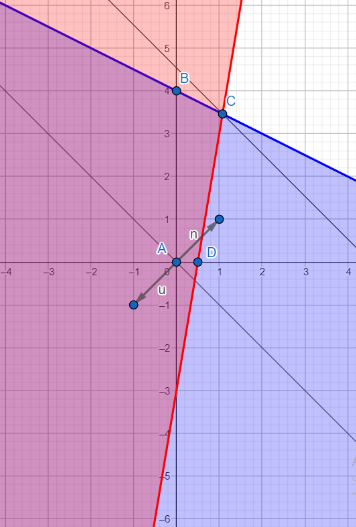
\includegraphics[]{пункт а.png}
\centering
\caption{График для решения задания №1, пункта 1a (построен с помощью \url{https://www.geogebra.org/calculator})}
\end{figure}

\begin{flushleft}
    Синяя область на графике - множество решений 1-го неравенства\\
    Красная область на графике - множество решений 2-го неравенства\\
    Область допустимых значений - четырехугольник ABCD\\
    $\vec{n}\{1; 1\}$ - $\nabla F$ (градиент)\\
    Если перемещать линию уровня (перпендикулярна $\vec{n}$, на графике отмечена серым цветом) в направлении $\vec{n}$, то после прохождения через точку С её пересечение с ОДЗ даёт пустое множество $\implies$ \\С - оптимальная точка задачи максимума\\
    Точка С является пересечением прямых $x_1 + 2x_2 = 8$ и $6x_1 - x_2 = 3 \implies$ координаты точки C являются решением системы:\\
    \begin{equation*}
        \begin{cases}
            x_1 + 2x_2 = 8 \\
            6x_1 - x_2 = 3 \\
        \end{cases}
    \end{equation*}
    Значит $C(\frac{14}{13}; \frac{45}{13}) \implies F_{max} = \frac{14}{13} + \frac{45}{13} = \frac{59}{13}$ \\
    Задача минимума сводится к задаче максимума для функции $G = -F = -x_1 - x_2$ \\
    $\vec{u}\{-1; -1\}$ - $\nabla G$ (градиент)\\
    Если перемещать линию уровня (перпендикулярна $\vec{u}$, на графике отмечена серым цветом) в направлении $\vec{u}$, то после прохождения через точку A её пересечение с ОДЗ даёт пустое множество $\implies$ \\A - оптимальная точка задачи максимума для функции G и, соответственно, задачи минимума для функции F\\
    $A(0; 0) \implies F_{min} = 0 + 0 = 0$
\end{flushleft}

{\bfОтвет:~} $F_{max} = F(\frac{14}{13}; \frac{45}{13}) = \frac{59}{13}$,  $F_{min} = F(0; 0) = 0$ 

\subsubsection{b)}
\begin{equation*}
    F = x_1 + 2x_2 \rightarrow max(min)
\end{equation*}
\begin{equation*}
    \begin{cases}
        x_1 + x_2 \ge 6 \\
        5x_1 - 10x_2 \le 10 \\
        x_1 \ge 0, x_2 \ge 0
    \end{cases}
\end{equation*}

\begin{center}
    {\bf
    Решение:}
\end{center}

\begin{figure}[ht]
\centering
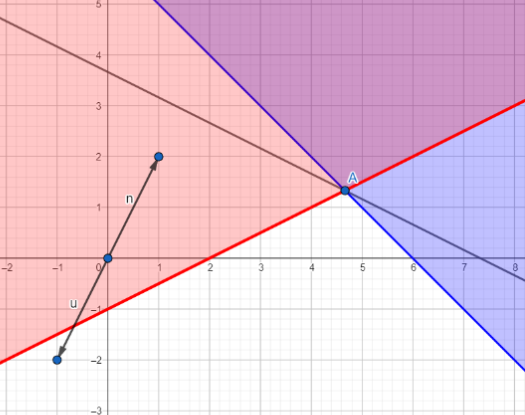
\includegraphics[]{пункт б.png}
\centering
\caption{График для решения задания №1, пункта 1b (построен с помощью \url{https://www.geogebra.org/calculator})}
\end{figure}

\begin{flushleft}
    Синяя область на графике - множество решений 1-го неравенства\\
    Красная область на графике - множество решений 2-го неравенства\\
    Область допустимых значений - часть области пересечения синей и красной областей, лежащая в первом квадранте\\
    $\vec{n}\{1; 2\}$ - $\nabla F$ (градиент)\\
    Область допустимых значений не ограничена в направлении $\vec{n} \implies F_{max}$ не определено\\
    Задача минимума сводится к задаче максимума для функции $G = -F = -x_1 - 2x_2$ \\
    $\vec{u}\{-1; -2\}$ - $\nabla G$ (градиент)\\
    Если перемещать линию уровня (перпендикулярна $\vec{u}$, на графике отмечена серым цветом) в направлении $\vec{u}$, то после прохождения через точку A её пересечение с ОДЗ даёт пустое множество $\implies$ \\A - оптимальная точка задачи максимума для функции G и, соответственно, задачи минимума для функции F\\
    Точка А является пересечением прямых $x_1 + x_2 = 6$ и $5x_1 - 10x_2 = 10 \implies$ координаты точки А являются решением системы:\\
    \begin{equation*}
        \begin{cases}
            x_1 + x_2 = 6 \\
            5x_1 - 10x_2 = 10 \\
        \end{cases}
    \end{equation*}
    Значит $A(\frac{14}{3}; \frac{4}{3}) \implies F_{min} = \frac{14}{3} + 2\cdot\frac{4}{3} = \frac{22}{3}$
\end{flushleft}

{\bfОтвет:~} $F_{max}$ не определено,  $F_{min} = F(\frac{14}{3}; \frac{4}{3}) = \frac{22}{3}$ 



\subsubsection{c)}
\begin{equation*}
    F = x_1 + 2x_2 \rightarrow max(min)
\end{equation*}
\begin{equation*}
    \begin{cases}
        2x_1 - x_2 \ge 6 \\
        2x_1 + x_2 \le 1 \\
        x_1 \ge 0, x_2 \ge 0
    \end{cases}
\end{equation*}

\begin{center}
    {\bf
    Решение:}
\end{center}

\begin{figure}[ht]
\centering
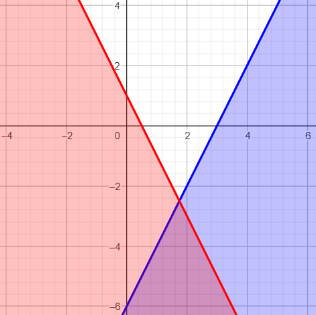
\includegraphics[]{пункт с.png}
\centering
\caption{График для решения задания №1, пункта 1c (построен с помощью \url{https://www.geogebra.org/calculator})}
\end{figure}


\begin{flushleft}
    Синяя область на графике - множество решений 1-го неравенства\\
    Красная область на графике - множество решений 2-го неравенства\\
    Точки, находящиеся в пересечении синей и красной областей, не удовлетворяют условиям $x_1 \ge 0$, $x_2 \ge 0$ $\implies$ область допустимых значений пустая $\implies F_{max}, F_{min}$ не определены
\end{flushleft}

{\bfОтвет:~} $F_{max}, F_{min}$ не определены

\chapter{Симплекс метод}

{\bf Вариант №1\\Найти решение задачи линейного программирования симплекс – методом (для "а, с" на max, для "в" на max и min)}

\subsubsection{a)}
\begin{equation*}
    F = x_1 + x_2 \rightarrow max
\end{equation*}
\begin{equation*}
    \begin{cases}
        x_1 + 2x_2 \le 8 \\
        6x_1 - x_2 \le 3 \\
        x_1 \ge 0, x_2 \ge 0
    \end{cases}
\end{equation*}

\begin{center}
    {\bf
    Решение:}
\end{center}

\begin{flushleft}
Приведем задачу к канонической форме:
\end{flushleft}

\begin{equation*}
    \begin{cases}
        x_1 + 2x_2 + x_3 = 8 \\
        6x_1 - x_2 + x_4 = 3 \\
        x_i \ge 0, i = 1, 2, 3, 4
    \end{cases}
\end{equation*}
\begin{center}
    $F - x_1 - x_2 = 0$
\end{center}

\begin{flushleft}
    {\bf1-я симплекс-таблица:}\\
\end{flushleft}

\begin{center}
    \begin{tabular}{|c | c g c c c c|} 
         \hline
            Базис & $x_1$ & $x_2$ & $x_3$ & $x_4$ & $b_i$ & $b_i/$р.с.\\
         \hline
         \rowcolor{LightBlue}
            $x_3$ & 1 & \cellcolor{cyan}2 & 1 & 0 & 8 & 8/2 = 4\\
         \hline
            $x_4$ & 6 & -1 & 0 & 1 & 3 & 3/(-1) = -3\\
         \hline
            F(x) & -1 & -1 & 0 & 0 & 0 &\\
         \hline
    \end{tabular}
\end{center}

\begin{flushleft}
    Наименьшее значение в строке F(x): -1\\
    Разрешающий столбец: $x_2$\\
    Минимальное положительное значение из столбца $b_i$/р.с. : 4\\
    Разрешающий элемент: 2\\
    Не все значения в строке F(x) положительные $\implies$ решение не оптимально, строим новую таблицу\\
    {\bf2-я симплекс-таблица:}\\
\end{flushleft}

\begin{center}
    \begin{tabular}{|c | g c c c c c|} 
         \hline
            Базис & $x_1$ & $x_2$ & $x_3$ & $x_4$ & $b_i$ & $b_i/$р.с.\\
         \hline
            $x_2$ & 1 & 2 & 1 & 0 & 8 & 8/1 = 8\\
         \hline
         \rowcolor{LightBlue}
            $x_4$ & \cellcolor{cyan}6.5 & 0 & 0.5 & 1 & 7 & 7/6.5 = $\frac{14}{13}$\\
         \hline
            F(x) & -0.5 & 0 & 0.5 & 0 & 4 &\\
         \hline
    \end{tabular}
\end{center}

\begin{flushleft}
    Наименьшее значение в строке F(x): -0.5\\
    Разрешающий столбец: $x_1$\\
    Минимальное положительное значение из столбца $b_i$/р.с. : $\frac{14}{13}$\\
    Разрешающий элемент: 6.5\\
    Не все значения в строке F(x) положительные $\implies$ решение не оптимально, строим новую таблицу\\
    {\bf3-я симплекс-таблица:}
\end{flushleft}

\begin{center}
    \begin{tabular}{|c | c c c c c c|} 
         \hline
            Базис & $x_1$ & $x_2$ & $x_3$ & $x_4$ & $b_i$ & $b_i/$р.с.\\
         \hline
            $x_2$ & 0 & 2 & $\frac{12}{13}$ & $-\frac{2}{13}$ & $\frac{90}{13}$ & \\
         \hline
            $x_1$ & 6.5 & 0 & 0.5 & 1 & 7 &\\
         \hline
            F(x) & 0 & 0 & $\frac{7}{13}$ & 1 & $\frac{59}{13}$ &\\
         \hline
    \end{tabular}
\end{center}

\begin{flushleft}
    Все значения в строке F(x) положительные, $F_{max}(x) = \frac{59}{13}$\\
    Оптимальное решение:\\
    $x_1 = 7:\frac{13}{2} = \frac{14}{13}$\\
    $x_2 = \frac{90}{13}:2 = \frac{45}{13}$
\end{flushleft}

{\bfОтвет:~} $F_{max} = F(\frac{14}{13}; \frac{45}{13}) = \frac{59}{13}$



\subsubsection{b)}
\begin{equation*}
    F = x_1 + 2x_2 \rightarrow max(min)
\end{equation*}
\begin{equation*}
    \begin{cases}
        x_1 + x_2 \ge 6 \\
        5x_1 - 10x_2 \le 10 \\
        x_1 \ge 0, x_2 \ge 0
    \end{cases}
\end{equation*}

\begin{center}
    {\bf
    Решение:}
\end{center}

\begin{flushleft}
Приведем задачу к канонической форме:
\end{flushleft}

\begin{equation*}
    \begin{cases}
        x_1 + x_2 - x_3 = 6 \\
        5x_1 - 10x_2 + x_4 = 10 \\
        x_i \ge 0, i = 1, 2, 3, 4
    \end{cases}
\end{equation*}
\begin{center}
    $F - x_1 - 2x_2 = 0$
\end{center}

\begin{flushleft}
    {\bf1. Задача на максимум}\\
    {\bf1-я симплекс-таблица:}\\
\end{flushleft}

\begin{center}
    \begin{tabular}{|c | c g c c c c|} 
         \hline
            Базис & $x_1$ & $x_2$ & $x_3$ & $x_4$ & $b_i$ & $b_i/$р.с.\\
         \hline
         \rowcolor{LightBlue}
            $x_3$ & 1 & \cellcolor{cyan}1 & -1 & 0 & 6 & 6/1 = 6\\
         \hline
            $x_4$ & 5 & -10 & 0 & 1 & 10 & 10/(-10) = -1\\
         \hline
            F(x) & -1 & -2 & 0 & 0 & 0 &\\
         \hline
    \end{tabular}
\end{center}

\begin{flushleft}
    Наименьшее значение в строке F(x): -2\\
    Разрешающий столбец: $x_2$\\
    Минимальное положительное значение из столбца $b_i$/р.с. : 6\\
    Разрешающий элемент: 1\\
    Не все значения в строке F(x) положительные $\implies$ решение не оптимально, строим новую таблицу\\
    {\bf2-я симплекс-таблица:}\\
\end{flushleft}

\begin{center}
    \begin{tabular}{|c | c c g c c c|} 
         \hline
            Базис & $x_1$ & $x_2$ & $x_3$ & $x_4$ & $b_i$ & $b_i/$р.с.\\
         \hline
            $x_2$ & 1 & 1 & -1 & 0 & 6 & 6/(-1) = -6\\
         \hline
            $x_4$ & 15 & 0 & -10 & 1 & 70 & 70/(-10) = -7\\
         \hline
            F(x) & 1 & 0 & -2 & 0 & 12 &\\
         \hline
    \end{tabular}
\end{center}

\begin{flushleft}
    Наименьшее значение в строке F(x): -2\\
    Разрешающий столбец: $x_3$\\
    Все значения в столбце $b_i$/р.с. отрицательные $\implies$ $F_{max}$ не определено
\end{flushleft}

\begin{flushleft}
    {\bf2. Задача на минимум}\\
\end{flushleft}

\begin{flushleft}
    В 1-й симплекс-таблице для задачи на максимум все значения в строке F(x) отрицательные $\implies$ оптимальное решение:\\
    $x_1 = 0$\\
    $x_2 = 6/(-1)$\\
    $x_3 = 0$\\
    $x_4 = 10/1 = 10$\\
    $x_2$ не удовлетворяет условию $x_2 \ge 0$ $\implies$ недопустимое решение\\
    {\bfПоставим вспомогательную задачу:}\\
\end{flushleft}

\begin{equation*}
    \begin{cases}
        x_1 + x_2 - x_3 + y_1= 6 \\
        5x_1 - 10x_2 + x_4 = 10 \\
        x_i \ge 0, i = 1, 2, 3, 4\\
        y_1 \ge 0
    \end{cases}
\end{equation*}
\begin{center}
    $G = - y_1 \rightarrow min$\\
    $G = y_1 \rightarrow max$
\end{center}

\begin{flushleft}
    {\bf1-я симплекс-таблица:}
\end{flushleft}

\begin{center}
    \begin{tabular}{|c | g c c c c c c|} 
         \hline
            Базис & $x_1$ & $x_2$ & $x_3$ & $x_4$ & $y_1$ & $b_i$ & $b_i/$р.с.\\
         \hline
            $y_1$ & 1 & 1 & -1 & 0 & 1 & 6 & 6/1 = 6\\
         \hline
         \rowcolor{LightBlue}
            $x_4$ & \cellcolor{cyan}5 & -10 & 0 & 1 & 0 & 10 & 10/5 = 2\\
         \hline
            $\Delta$ & -1 & -1 & 1 & 0 & 0 & $G = 6$ &\\
         \hline
    \end{tabular}
\end{center}

\begin{flushleft}
    Наибольшая положительная $\Delta$: 1\\
    Разрешающий столбец: $x_1$\\
    Минимальное положительное значение из столбца $b_i$/р.с. : 2\\
    Разрешающий элемент: 5\\
    Не все $\Delta > 0$ $\implies$ решение не оптимально, строим новую таблицу\\
    {\bf2-я симплекс-таблица:}\\
\end{flushleft}

\begin{center}
    \begin{tabular}{|c | c g c c c c c|} 
         \hline
            Базис & $x_1$ & $x_2$ & $x_3$ & $x_4$ & $y_1$ & $b_i$ & $b_i/$р.с.\\
         \hline
         \rowcolor{LightBlue}
            $y_1$ & 0 & \cellcolor{cyan}3 & -1 & -0.2 & 1 & 4 & 4/3 = $\frac{4}{3}$\\
         \hline
            $x_1$ & 5 & -10 & 0 & 1 & 0 & 10 & 10/(-10) = -1\\
         \hline
            $\Delta$ & 0 & -3 & 1 & 0.2 & 0 & $G = 8$ &\\
         \hline
    \end{tabular}
\end{center}

\begin{flushleft}
    Наибольшая положительная $\Delta$: 3\\
    Разрешающий столбец: $x_2$\\
    Минимальное положительное значение из столбца $b_i$/р.с. : $\frac{4}{3}$\\
    Разрешающий элемент: 3\\
    Не все $\Delta > 0$ $\implies$ решение не оптимально, строим новую таблицу\\
    {\bf3-я симплекс-таблица:}\\
\end{flushleft}

\begin{center}
    \begin{tabular}{|c | c c c c c c c|} 
         \hline
            Базис & $x_1$ & $x_2$ & $x_3$ & $x_4$ & $y_1$ & $b_i$ & $b_i/$р.с.\\
         \hline
            $x_2$ & 0 & 3 & -1 & -0.2 & 1 & 4 &\\
         \hline
            $x_1$ & 5 & 0 & -$\frac{10}{3}$ & $\frac{1}{3}$ & $\frac{10}{3}$ & $\frac{70}{3}$ &\\
         \hline
            $\Delta$ & 0 & 0 & 0 & 0 & 1 & $G = 12$ &\\
         \hline
    \end{tabular}
\end{center}

\begin{flushleft}
    Все $\Delta > 0$ $\implies$ решение оптимально\\
    $x_1 = \frac{70}{3} : 5 = \frac{14}{3}$\\
    $x_2 = 4 : 3 = \frac{4}{3}$\\
    $F_{min} = \frac{14}{3} + 2 \cdot \frac{4}{3} = \frac{22}{3}$ 
\end{flushleft}

{\bfОтвет:~} $F_{max}$ не определено; $F_{min} = F(\frac{14}{3}; \frac{4}{3}) = \frac{22}{3}$


\subsubsection{c)}
\begin{equation*}
    F = x_1 + 2x_2 \rightarrow max
\end{equation*}
\begin{equation*}
    \begin{cases}
        2x_1 - x_2 \ge 6 \\
        2x_1 + x_2 \le 1 \\
        x_1 \ge 0, x_2 \ge 0
    \end{cases}
\end{equation*}

\begin{center}
    {\bf
    Решение:}
\end{center}

\begin{flushleft}
Приведем задачу к канонической форме:
\end{flushleft}

\begin{equation*}
    \begin{cases}
        2x_1 - x_2 - x_3 = 6 \\
        2x_1 + x_2 + x_4 = 1 \\
        x_i \ge 0, i = 1, 2, 3, 4
    \end{cases}
\end{equation*}
\begin{center}
    $F - x_1 - 2x_2 = 0$
\end{center}

\begin{flushleft}
    {\bf1-я симплекс-таблица:}\\
\end{flushleft}

\begin{center}
    \begin{tabular}{|c | c g c c c c|} 
         \hline
            Базис & $x_1$ & $x_2$ & $x_3$ & $x_4$ & $b_i$ & $b_i/$р.с.\\
         \hline
            $x_3$ & 2 & -1 & -1 & 0 & 6 & 6/(-1) = -6\\
         \hline
         \rowcolor{LightBlue}
            $x_4$ & 2 & \cellcolor{cyan}1 & 0 & 1 & 1 & 1/1 = 1\\
         \hline
            F(x) & -1 & -2 & 0 & 0 & 0 &\\
         \hline
    \end{tabular}
\end{center}

\begin{flushleft}
    Наименьшее значение в строке F(x): -2\\
    Разрешающий столбец: $x_2$\\
    Минимальное положительное значение из столбца $b_i$/р.с. : 1\\
    Разрешающий элемент: 1\\
    Не все значения в строке F(x) положительные $\implies$ решение не оптимально, строим новую таблицу\\
    {\bf2-я симплекс-таблица:}\\
\end{flushleft}

\begin{center}
    \begin{tabular}{|c | c c c c c c|} 
         \hline
            Базис & $x_1$ & $x_2$ & $x_3$ & $x_4$ & $b_i$ & $b_i/$р.с.\\
         \hline
            $x_3$ & 4 & 0 & -1 & 1 & 7 &\\
         \hline
            $x_2$ & 2 & 1 & 0 & 1 & 1 & \\
         \hline
            F(x) & 3 & 0 & 0 & 2 & 2 &\\
         \hline
    \end{tabular}
\end{center}

\begin{flushleft}
    Все значения в строке F(x) положительные\\
    Оптимальное решение:\\
    $x_1 = 0$\\
    $x_2 = 1/1 = 1$\\
    $x_3 = 7/(-1)$\\
    $x_4 = 0$\\
    $x_3$ не удовлетворяет условию $x_3 \ge 0$ $\implies$ недопустимое решение\\
    {\bfПоставим вспомогательную задачу:}\\
\end{flushleft}

\begin{equation*}
    \begin{cases}
        2x_1 - x_2 - x_3 + y_1= 6 \\
        2x_1 + x_2 + x_4 = 1 \\
        x_i \ge 0, i = 1, 2, 3, 4\\
        y_1 \ge 0
    \end{cases}
\end{equation*}
\begin{center}
    $G = - y_1 \rightarrow max$
\end{center}


\begin{flushleft}
    {\bf1-я симплекс-таблица:}
\end{flushleft}

\begin{center}
    \begin{tabular}{|c | g c c c c c c|} 
         \hline
            Базис & $x_1$ & $x_2$ & $x_3$ & $x_4$ & $y_1$ & $b_i$ & $b_i/$р.с.\\
         \hline
            $y_1$ & 2 & -1 & -1 & 0 & 1 & 6 & 6/(-1) = -6\\
         \hline
         \rowcolor{LightBlue}
            $x_4$ & \cellcolor{cyan}2 & 1 & 0 & 1 & 0 & 1 & 1/1 = 1\\
         \hline
            $\Delta$ & 2 & -1 & -1 & 0 & 0 & $G = -6$ &\\
         \hline
    \end{tabular}
\end{center}

\begin{flushleft}
    Наибольшая положительная $\Delta$: 2\\
    Разрешающий столбец: $x_1$\\
    Минимальное положительное значение из столбца $b_i$/р.с. : 1\\
    Разрешающий элемент: 2\\
    Не все $\Delta < 0$ $\implies$ решение не оптимально, строим новую таблицу\\
    {\bf2-я симплекс-таблица:}\\
\end{flushleft}

\begin{center}
    \begin{tabular}{|c | c c c c c c c|} 
         \hline
            Базис & $x_1$ & $x_2$ & $x_3$ & $x_4$ & $y_1$ & $b_i$ & $b_i/$р.с.\\
         \hline
            $y_1$ & 0 & -2 & -1 & -1 & 1 & 5 & 6/(-1) = -6\\
         \hline
            $x_1$ & 2 & 1 & 0 & 1 & 0 & 1 & 1/1 = 1\\
         \hline
            $\Delta$ & 0 & -2 & -1 & -1 & 0 & $G = -7$ &\\
         \hline
    \end{tabular}
\end{center}

\begin{flushleft}
    Все $\Delta < 0, G < 0 \implies $ в исходной задаче область допустимых значений пустая $\implies F_{max} $ не определено 
\end{flushleft}

{\bfОтвет:~} $F_{max}$ не определено

\chapter{Двойственная задача}

{\bf Вариант №1\\ Для "а" составить и решить геометрически и симплекс – методом задачу двойственную данной.}

\begin{center}
    {\bf
    Решение:}
\end{center}

\subsubsection{1) Нахождение минимума двойственной задачи}

\begin{flushleft}
Прямая задача на максимум:
\end{flushleft}

\begin{equation*}
    F = x_1 + x_2 \rightarrow max
\end{equation*}
\begin{equation*}
    \begin{cases}
        x_1 + 2x_2 \le 8 \\
        6x_1 - x_2 \le 3 \\
        x_1 \ge 0, x_2 \ge 0
    \end{cases}
\end{equation*}

\begin{flushleft}
Из пункта 1а $\implies x_{max} = (\frac{14}{13}; \frac{45}{13}), F_{max} = \frac{59}{13}$
\end{flushleft}

\begin{flushleft}
Поставим двойственную задачу:
\end{flushleft}

\begin{center}
    $F^{*} = 8y_1 + 3y_2 \rightarrow min$
\end{center}
\begin{equation*}
    \begin{cases}
        y_1 + 6y_2 \ge 1\\
        2y_1 - y_2 \ge 1\\
        y_i \ge 0, i = 1, 2\\
    \end{cases}
\end{equation*}

\subsubsection{1.1) Решение с помощью теоремы 2}

\begin{equation*}
    \begin{cases}
        (1 \cdot x_1^{*} + 2 \cdot x_2^{*} - 8)y_1^{*} = 0\\
        (6 \cdot x_1^{*} - x_2^{*} - 3)y_2^{*} = 0\\
        (y_1^{*} + 6y_2^{*} - 1)x_1^{*} = 0\\
        (2y_1^{*} - y_2^{*} - 1)x_2^{*} = 0\\
    \end{cases}
\end{equation*}

\begin{equation*}
    \begin{cases}
        (1 \cdot \frac{14}{13} + 2 \cdot \frac{45}{13} - 8)y_1^{*} = 0\\
        (6 \cdot \frac{14}{13} - \frac{45}{13} - 3)y_2^{*} = 0\\
        (y_1^{*} + 6y_2^{*} - 1) \cdot \frac{14}{13} = 0\\
        (2y_1^{*} - y_2^{*} - 1) \cdot \frac{45}{13} = 0\\
    \end{cases}
\end{equation*}

\begin{equation*}
    \begin{cases}
        0 \cdot y_1^{*} = 0\\
        0 \cdot y_2^{*} = 0\\
        y_1^{*} + 6y_2^{*} - 1 = 0\\
        2y_1^{*} - y_2^{*} - 1 = 0\\
    \end{cases}
\end{equation*}

\begin{equation*}
    \begin{cases}
        y_1^{*} > 0\\
        y_2^{*} > 0\\
        y_1^{*} + 6y_2^{*} - 1 = 0\\
        2y_1^{*} - y_2^{*} - 1 = 0\\
    \end{cases}
\end{equation*}

\begin{flushleft}
В результате решения системы получим:
\end{flushleft}
\begin{equation*}
    \begin{cases}
        y_1^{*} = \frac{7}{13}\\
        y_2^{*} = \frac{1}{13}\\
    \end{cases}
\end{equation*}

\begin{flushleft}
$F_{min}^{*} = F^{*}(\frac{7}{13}; \frac{1}{13}) = 8 \cdot \frac{7}{13} + 3 \cdot \frac{1}{13} = \frac{59}{13}$
\end{flushleft}

{\bfОтвет:~} $F_{min}^{*} = F^{*}(\frac{7}{13}; \frac{1}{13}) = \frac{59}{13} = F_{max}$

\subsubsection{1.2) Решение с помощью теоремы 3}

\begin{flushleft}
В пункте 2а была получена итоговая симплекс-таблица:    
\end{flushleft}

\begin{center}
    \begin{tabular}{|c | c c c c c|} 
         \hline
            Базис & $x_1$ & $x_2$ & $x_3$ & $x_4$ & $b_i$\\
         \hline
            $x_2$ & 0 & 2 & $\frac{12}{13}$ & $-\frac{2}{13}$ & $\frac{90}{13}$\\
         \hline
            $x_1$ & 6.5 & 0 & 0.5 & 1 & 7\\
         \hline
            F(x) & 0 & 0 & $\frac{7}{13}$ & 1 & $\frac{59}{13}$\\
         \hline
    \end{tabular}
\end{center}

\begin{flushleft}
Поделим строку, соответствующую $x_2$, на 2; строку, соответствующую $x_1$, на 6.5. Добавим в таблицу столбец $C_{B}$,значениями которого являются коэффициенты при соответствующих $x_i$ в F(x):
\end{flushleft}

\begin{center}
    \begin{tabular}{|c | c c c c c c|} 
         \hline
            Базис & $x_1$ & $x_2$ & $x_3$ & $x_4$ & $b_i$ & $C_{B}$\\
         \hline
            $x_2$ & 0 & 1 & $\frac{6}{13}$ & $-\frac{1}{13}$ & $\frac{45}{13}$ & 1\\
         \hline
            $x_1$ & 1 & 0 & $\frac{1}{13}$ & $\frac{2}{13}$ & $\frac{14}{13}$ & 1\\
         \hline
            F(x) & 0 & 0 & $\frac{7}{13}$ & 1 & $\frac{59}{13}$ &\\
         \hline
    \end{tabular}
\end{center}

\begin{flushleft}
$y^{*} = C_{B} \cdot A_{B}^{-1} = (1; 1) \cdot \begin{pmatrix}
\frac{6}{13} & -\frac{1}{13} \\
\frac{1}{13} & \frac{2}{13} \\
\end{pmatrix} = (\frac{6}{13} + \frac{1}{13}; -\frac{1}{13} + \frac{2}{13}) = (\frac{7}{13}; \frac{1}{13})$ \\
$F_{min}^{*} = F^{*}(\frac{7}{13}; \frac{1}{13}) = 8 \cdot \frac{7}{13} + 3 \cdot \frac{1}{13} = \frac{59}{13}$
\end{flushleft}

{\bfОтвет:~} $F_{min}^{*} = F^{*}(\frac{7}{13}; \frac{1}{13}) = \frac{59}{13} = F_{max}$



\subsubsection{2) Нахождение максимума двойственной задачи}

\begin{flushleft}
Прямая задача на минимум:
\end{flushleft}

\begin{equation*}
    F = x_1 + x_2 \rightarrow min
\end{equation*}
\begin{equation*}
    \begin{cases}
        x_1 + 2x_2 \le 8 \\
        6x_1 - x_2 \le 3 \\
        x_1 \ge 0, x_2 \ge 0
    \end{cases}
\end{equation*}

\begin{flushleft}
Из пункта 1а $\implies x_{min} = (0; 0), F_{min} = 0$
\end{flushleft}

\begin{flushleft}
Поставим двойственную задачу:
\end{flushleft}

\begin{center}
    $F^{*} = 8y_1 + 3y_2 \rightarrow max$
\end{center}
\begin{equation*}
    \begin{cases}
        y_1 + 6y_2 \ge 1\\
        2y_1 - y_2 \ge 1\\
        y_i \ge 0, i = 1, 2\\
    \end{cases}
\end{equation*}

\subsubsection{2.1) Решение с помощью теоремы 2}

\begin{equation*}
    \begin{cases}
        (1 \cdot x_1^{*} + 2 \cdot x_2^{*} - 8)y_1^{*} = 0\\
        (6 \cdot x_1^{*} - x_2^{*} - 3)y_2^{*} = 0\\
        (y_1^{*} + 6y_2^{*} - 1)x_1^{*} = 0\\
        (2y_1^{*} - y_2^{*} - 1)x_2^{*} = 0\\
    \end{cases}
\end{equation*}

\begin{equation*}
    \begin{cases}
        (1 \cdot 0 + 2 \cdot 0 - 8)y_1^{*} = 0\\
        (6 \cdot 0 - 0 - 3)y_2^{*} = 0\\
        (y_1^{*} + 6y_2^{*} - 1) \cdot 0 = 0\\
        (2y_1^{*} - y_2^{*} - 1) \cdot 0 = 0\\
    \end{cases}
\end{equation*}

\begin{equation*}
    \begin{cases}
        y_1^{*} = 0\\
        y_2^{*} = 0\\
    \end{cases}
\end{equation*}

\begin{flushleft}
$F_{max}^{*} = F^{*}(0; 0) = 8 \cdot 0 + 3 \cdot 0 = 0$
\end{flushleft}

{\bfОтвет:~} $F_{max}^{*} = F^{*}(0; 0) = 0 = F_{min}$

\subsubsection{2.2) Решение с помощью теоремы 3}

\begin{flushleft}
Первая симплекс-таблица в пункте 2а является итоговой симплекс-таблицей для прямой задачи на минимум:
\end{flushleft}

\begin{center}
    \begin{tabular}{|c | c c c c c|} 
         \hline
            Базис & $x_1$ & $x_2$ & $x_3$ & $x_4$ & $b_i$\\
         \hline
            $x_3$ & 1 & 2 & 1 & 0 & 8\\
         \hline
            $x_4$ & 6 & -1 & 0 & 1 & 3\\
         \hline
            F(x) & -1 & -1 & 0 & 0 & 0\\
         \hline
    \end{tabular}
\end{center}

\begin{flushleft}
Добавим в таблицу столбец $C_{B}$, значениями которого являются коэффициенты при соответствующих $x_i$ в F(x):
\end{flushleft}

\begin{center}
    \begin{tabular}{|c | c c c c c c|} 
         \hline
            Базис & $x_1$ & $x_2$ & $x_3$ & $x_4$ & $b_i$ & $C_{B}$\\
         \hline
            $x_3$ & 1 & 2 & 1 & 0 & 8 & 0\\
         \hline
            $x_4$ & 6 & -1 & 0 & 1 & 3 & 0\\
         \hline
            F(x) & -1 & -1 & 0 & 0 & 0 &\\
         \hline
    \end{tabular}
\end{center}

\begin{flushleft}
$y^{*} = C_{B} \cdot A_{B}^{-1} = (0; 0) \cdot \begin{pmatrix}
1 & 0 \\
0 & 1 \\
\end{pmatrix} = (0; 0)$ \\
$F_{min}^{*} = F^{*}(0; 0) = 8 \cdot 0 + 3 \cdot 0 = 0$
\end{flushleft}

{\bfОтвет:~} $F_{max}^{*} = F^{*}(0; 0) = 0 = F_{min}$

\chapter{Экономическая задача}
{\bfВариант 12}
\begin{flushleft}
    Составить математическую модель для прямой и двойственной задачи. Получить решение прямой и двойственной задачи симплекс-методом. Дать экономическую интерпретацию двойственных задач и двойственных оценок.\\
    Для производства четырех видов изделий (А, В, С) предприятие использует три вида сырья: металл, пластмассу, резину. Запасы сырья, технологические коэффициенты (расход каждого вида сырья на производство единицы каждого изделия) представлены в таблице. В ней же указана прибыль от реализации одного изделия каждого вида. Требуется составить такой план выпуска указанных изделий, чтобы обеспечить максимальную прибыль.
\end{flushleft}

\begin{center}
    \begin{tabular}{|c | c | c | c | c | c|} 
         \hline
            & A & B & C & D & запасы\\
         \hline
            металл & 3 & 0 & 1 & 1 & 1000\\
         \hline
            пластмасса & 6 & 4 & 2 & 1 & 1100\\
         \hline
            резина & 9 & 12 & 2 & 5 & 1300\\
         \hline
            прибыль (руб) & 9 & 7 & 2 & 6 & \\
        \hline
    \end{tabular}
\end{center}

\begin{center}
    {\bf
    Решение:}
\end{center}

{\bf1. Постановка задачи}\\
{\bf1.1. Постановка прямой задачи:}
\begin{flushleft}
    Найти оптимальный план производства продукции с максимальной прибылью, для которого достаточно имеющихся ресурсов. $x_1, x_2, x_3, x_4$ – количество произведенной продукции.\\
\end{flushleft}
Целевая функция прямой задачи:
\begin{equation*}
    F = 9x_1 + 7x_2 + 2x_3 + 6x_4 \rightarrow max
\end{equation*}
Ограничения прямой задачи:
\begin{equation*}
    \begin{cases}
        3x_1 + x_3 + x_4 \le 1000 \\
        6x_1 + 4x_2 + 2x_3 + x_4 \le 1100 \\
        9x_1 + 12x_2 + 2x_3 + 5x_4 \le 1300 \\
        x_i \ge 0, i = 1, 2, 3, 4
    \end{cases}
\end{equation*}

{\bf1.2. Постановка двойственной задачи:}
\begin{flushleft}
    Оценить каждый из видов сырья, используемого для производства продукции. Оценки, приписываемые каждому виду сырья, должны быть такими, чтобы оценка всего используемого сырья была минимальна, а суммарная оценка сырья, используемого для производства единицы продукции – не меньше цены единицы продукции.
\end{flushleft}
Целевая функция двойственной задачи:
\begin{equation*}
    G = 1000y_1 + 1100y_2 + 1300y_3 \rightarrow min
\end{equation*}
Ограничения двойственной задачи:
\begin{equation*}
    \begin{cases}
        3y_1 + 6y_2 + 9y_3 \ge 9 \\
        4y_2 + 12y_3 \ge 7 \\
        y_1 + 2y_2 + 2y_3 \ge 2 \\
        y_1 + y_2 + 5y_3 \ge 6 \\
        y_i \ge 0, i = 1, 2, 3
    \end{cases}
\end{equation*}
{\bf2. Решим прямую задачу}, введя 3 фиктивные переменные: $x_5, x_6, x_7$\\
Канонический вид прямой задачи:

\begin{equation*}
    \begin{cases}
        3x_1 + x_3 + x_4 + x_5 = 1000 \\
        6x_1 + 4x_2 + 2x_3 + x_4 + x_6 = 1100 \\
        9x_1 + 12x_2 + 2x_3 + 5x_4 + x_7 = 1300 \\
        x_i \ge 0, i = 1, 2, 3, 4, 5, 6, 7
    \end{cases}
\end{equation*}
\begin{equation*}
    F - 9x_1 - 7x_2 - 2x_3 - 6x_4 = 0
\end{equation*}

\begin{flushleft}
    {\bf1-я симплекс-таблица:}\\
\end{flushleft}

\begin{center}
    \begin{tabular}{|c | g c c c c c c c c|} 
         \hline
            Базис & $x_1$ & $x_2$ & $x_3$ & $x_4$ & $x_5$ & $x_6$ & $x_7$ & $b_i$ & $b_i/$р.с.\\
         \hline
            $x_5$ & 3 & 0 & 1 & 1 & 1 & 0 & 0 & 1000 & $\frac{1000}{3}$\\
         \hline
            $x_6$ & 6 & 4 & 2 & 1 & 0 & 1 & 0 & 1100 & $\frac{550}{3}$ \\
        \hline
        \rowcolor{LightBlue}
            $x_7$ & \cellcolor{cyan}9 & 12 & 2 & 5 & 0 & 0 & 1 & 1300 & $\frac{1300}{9}$ \\
         \hline
            F(x) & -9 & -7 & -2 & -6 & 0 & 0 & 0 & 0 &\\
         \hline
    \end{tabular}
\end{center}

\begin{flushleft}
    Наименьшее значение в строке F(x): -9\\
    Разрешающий столбец: $x_1$\\
    Минимальное положительное значение из столбца $b_i$/р.с. : $\frac{1300}{9}$\\
    Разрешающий элемент: 9\\
    Не все значения в строке F(x) положительные $\implies$ решение не оптимально, строим новую таблицу\\
    {\bf2-я симплекс-таблица:}\\
\end{flushleft}

\begin{center}
    \begin{tabular}{|c | c c c g c c c c c|} 
         \hline
            Базис & $x_1$ & $x_2$ & $x_3$ & $x_4$ & $x_5$ & $x_6$ & $x_7$ & $b_i$ & $b_i/$р.с.\\
         \hline
            $x_5$ & 0 & -4 & $\frac{1}{3}$ & $-\frac{2}{3}$ & 1 & 0 & $-\frac{1}{3}$ & $\frac{1700}{3}$ & -850 \\
         \hline
            $x_6$ & 0 & -4 & $\frac{2}{3}$ & $-\frac{7}{3}$ & 0 & 1 & $-\frac{2}{3}$ & $\frac{700}{3}$ & -100 \\
        \hline
        \rowcolor{LightBlue}
            $x_1$ & 9 & 12 & 2 & \cellcolor{cyan}5 & 0 & 0 & 1 & 1300 & 260 \\
         \hline
            F(x) & 0 & 5 & 0 & -1 & 0 & 0 & 1 & 1300 & -1300\\
         \hline
    \end{tabular}
\end{center}

\begin{flushleft}
    Наименьшее значение в строке F(x): -1\\
    Разрешающий столбец: $x_4$\\
    Минимальное положительное значение из столбца $b_i$/р.с. : 260\\
    Разрешающий элемент: 5\\
    Не все значения в строке F(x) положительные $\implies$ решение не оптимально, строим новую таблицу\\
    {\bf3-я симплекс-таблица:}\\
\end{flushleft}

\begin{center}
    \begin{tabular}{|c | c c c c c c c c c|} 
         \hline
            Базис & $x_1$ & $x_2$ & $x_3$ & $x_4$ & $x_5$ & $x_6$ & $x_7$ & $b_i$ & $C_{B}$\\
         \hline
            $x_5$ & $\frac{6}{5}$ & $-\frac{12}{5}$ & $\frac{3}{5}$ & 0 & 1 & 0 & $-\frac{1}{5}$ & 740 & 0 \\
         \hline
            $x_6$ & $\frac{21}{5}$ & $\frac{8}{5}$ & $\frac{19}{15}$ & 0 & 0 & 1 & $-\frac{1}{5}$ & 840 & 0 \\
        \hline
            $x_4$ & 9 & 12 & 2 & 5 & 0 & 0 & 1 & 1300 & 6 \\
         \hline
            F(x) & $\frac{9}{5}$ & $\frac{37}{5}$ & $\frac{2}{5}$ & 0 & 0 & 0 & $\frac{6}{5}$ & 1560 & \\
         \hline
    \end{tabular}
\end{center}

\begin{flushleft}
    Все значения в строке F(x) положительные $\implies$ решение оптимально\\
    {\bf$x^{*} = (0, 0, 0, 260, 740, 840, 0)$ - оптимальное решение\\
    $F_{max} = F(x^{*}) = 1560$\\
    $y^{*} = (0, 0, \frac{6}{5}, \frac{9}{5}, \frac{37}{5}, \frac{2}{5}, 0)$}\\
\end{flushleft}

{\bf3. Решим двойственную задачу:}\\
{\bf3.1. Решение через условия дополняющей нежесткости.}\\
По 2-й теореме двойственности оптимальное решение двойственной задачи удовлетворяет условиям:
\begin{equation*}
    \begin{cases}
        \displaystyle\sum_{j=1}^{n} (a_{ij} \cdot x_{j}^{*} - b_{i}) \cdot y_{i}^{*} = 0, i = \overline{1, m}\\
        \displaystyle\sum_{i=1}^{m} (a_{ij} \cdot y_{i}^{*} - c_{j}) \cdot x_{j}^{*} = 0, j = \overline{1, n}
    \end{cases}
\end{equation*}
\begin{equation*}
    \begin{cases}
        (3 \cdot 0 + 1 \cdot 0 + 1 \cdot 260 - 1000) \cdot y_{1}^{*} = 0\\
        (6 \cdot 0 + 4 \cdot 0 + 2 \cdot 0 + 1 \cdot 260 - 1100) \cdot y_{2}^{*} = 0\\
        (9 \cdot 0 + 12 \cdot 0 + 2 \cdot 0 + 5 \cdot 260 - 1300) \cdot y_{3}^{*} = 0\\
        (3 \cdot y_{1}^{*} + 6 \cdot y_{2}^{*} + 9 \cdot y_{3}^{*} - 9) \cdot 0 = 0\\
        (4 \cdot y_{2}^{*} + 12 \cdot y_{3}^{*} - 7) \cdot 0 = 0\\
        (1 \cdot y_{1}^{*} + 2 \cdot y_{2}^{*} + 2 \cdot y_{3}^{*} - 2) \cdot 0 = 0\\
        (1 \cdot y_{1}^{*} + 1 \cdot y_{2}^{*} + 5 \cdot y_{3}^{*} - 6) \cdot 260 = 0
    \end{cases}
\end{equation*}
\begin{equation*}
    \begin{cases}
        y_{1}^{*} = 0\\
        y_{2}^{*} = 0\\
        y_{3}^{*} = \frac{6}{5}
    \end{cases}
\end{equation*}
{\bf3.2. Решение по формуле: $y^{*} = C_{B} \cdot A_{B}^{-1}$}
\begin{flushleft}
    $y^{*} = C_{B} \cdot A_{B}^{-1} = (0; 0; 6) \cdot \begin{pmatrix}
1 & 0 & -\frac{1}{5} \\
0 & 1 & -\frac{1}{5}\\
0 & 0 & \frac{1}{5}\\
\end{pmatrix} = (0; 0; \frac{6}{5})$
\end{flushleft}

{\bf4. Анализ результатов}\\
$x_5, x_6, x_7$ - остатки сырья\\
{\bf4.1. Подставим $x^{*}$ в ограничения прямой задачи:}

\begin{equation*}
    \begin{cases}
        3 \cdot 0 + 0 + 260 = 260 \le 1000 \\
        6 \cdot 0 + 4 \cdot 0 + 2 \cdot 0 + 260 = 260 \le 1100 \\
        9 \cdot 0 + 12 \cdot 0 + 2 \cdot 0 + 5 \cdot 260 = 1300 \\
    \end{cases}
\end{equation*}

\begin{flushleft}
    1) 1-е, 2-е условия имеют знак "<", значит 1-й и 2-й ресурсы (металл и пластмасса) не являются дефицитными, их остатки соответственно равны $x^{*}_5 = 740$, $x^{*}_6 = 840$\\
    2) 3-е условие имеет знак "=", значит 3-й ресурс (резина) дефицитный ($x_7 = 0$)
\end{flushleft}
\begin{flushleft}
    Положительную двойственную оценку имеют только дефицитные виды сырья
\end{flushleft}

{\bf4.2. Подставим $y^{*}$ в ограничения двойственной задачи:}

\begin{equation*}
    \begin{cases}
        3 \cdot 0 + 6 \cdot 0 + 9 \cdot \frac{6}{5} = \frac{54}{5} \ge 9 \\
        4 \cdot 0 + 12 \cdot \frac{6}{5} = \frac{72}{5} \ge 7 \\
        0 + 2 \cdot 0 + 2 \cdot \frac{6}{5} = \frac{12}{5} \ge 2 \\
        0 + 0 + 5 \cdot \frac{6}{5} = 6 \\
    \end{cases}
\end{equation*}

\begin{flushleft}
    1) 4-е ограничение имеет знак "=", значит двойственная оценка ресурса, используемого для изготовления изделия вида D в точности равна доходам, а значит изделия производить целесообразно\\
    2) 1-е, 2-е, 3-е ограничения имеют знак ">", значит производить изделия A, B, C нецелесообразно
\end{flushleft}

{\bf4.3.}
    Величина двойственных оценок показывает, насколько возрастет значение целевой функции при увеличении запасов дефицитного ресурса на одну единицу.\\
    Увеличение запасов 3-го ресурса (резина) на единицу приведет к новому оптимальному плану: $F_{max} = 1561.2$
    Коэффициент $A_{b}^{-1}$ показывают, что увеличение прибыли достигается засчет увеличения выпуска продукции D на 0.2 единицы; при этом запасы металла и пластмассы сократятся на 0.2 единиц соответственно 

{\bf5. Анализ устойчивости двойственных оценок}
\newline
Определим интервалы устойчивости:\\
$x_{b new}^{*} = x_{b} + A_{b}^{-1} \cdot \Delta b = A_{b}^{-1} \cdot (b + \Delta b)$\\
$A_{b}^{-1} \cdot (b + \Delta b) \ge 0$

$A_{b}^{-1} \cdot (b + \Delta b) = \begin{pmatrix}
1 & 0 & -\frac{1}{5} \\
0 & 1 & -\frac{1}{5}\\
0 & 0 & \frac{1}{5}\\
\end{pmatrix}
\begin{pmatrix}
1000 + \Delta b_1 \\
1100 + \Delta b_2 \\
1300 + \Delta b_3 \\
\end{pmatrix} = \begin{pmatrix}
740 + \Delta b_1 - \frac{1}{5} \Delta b_3 \\
840 + \Delta b_2 - \frac{1}{5} \Delta b_3 \\
260 + \frac{1}{5} \Delta b_3 \\
\end{pmatrix} \ge 0$\\
Частные случаи:\\
1) $\Delta b_2 = \Delta b_3 = 0 \implies \Delta b_1 \ge -740 \implies$ запасы 1-го ресурса можно уменьшать не более чем на 740 единиц, при этом оптимальный план двойственной задачи не изменится.\\
2) $\Delta b_1 = \Delta b_3 = 0 \implies \Delta b_2 \ge -840 \implies$ запасы 2-го ресурса можно уменьшать не более чем на 840 единиц, при этом оптимальный план двойственной задачи не изменится.\\
3) $\Delta b_1 = \Delta b_2 = 0 \implies \Delta b_3 \in [-1300; 3700] \implies$ при увеличении запасов 3-го ресурса не более чем на 3700 единиц и уменьшении его запасов не более чем на 1300 единиц значение целевой функции не изменится.\\

Предположим, что $\Delta b_2 = -100, \Delta b_3 = -200$. Тогда:\\
$\begin{pmatrix}
x_5^{new}\\
x_6^{new}\\
x_4^{new}\\
\end{pmatrix} = \begin{pmatrix}
740 + \frac{1}{5} \cdot 200 \\
840 - 100 + \frac{1}{5} \cdot 200 \\
260 - \frac{1}{5} \cdot 200 \\
\end{pmatrix} \ge 0 \implies \Delta b_2, \Delta b_3$ сохраняют оценки ресурсов в пределах устойчивости.
$x_{new} = (0; 0; 0; 220; 780; 780; 0)$\\
Целевая функция изменится на 240 и станет равной $F_{new} = 6 \cdot 220 = 1320$

\chapter{Транспортная задача}

Решить транспортную задачу с m = 3 поставщиками и n = 7 потребителями. Данные о запасах, спросе и стоимости транспортировки приведены в таблице.

\begin{center}
    \begin{tabular}{|a | c | c | c | c | c | c | c | c|} 
         \hline
         \rowcolor{LightGray}
            & 1 & 2 & 3 & 4 & 5 & 6 & 7 & запасы\\
         \hline
            1 & 5 & 8 & 1 & 4 & 2 & 7 & 3 & 150\\
         \hline
            2 & 3 & 6 & 4 & 9 & 1 & 8 & 2 & 100\\
         \hline
            3 & 7 & 1 & 5 & 8 & 3 & 2 & 4 & 150\\
         \hline
            спрос & 60 & 40 & 70 & 50 & 90 & 40 & 50 & $\sum =$ 400\\
        \hline
    \end{tabular}
\end{center}

\begin{center}
    {\bf
    Решение:}
\end{center}

$5x_{11} + 8x_{12} + x_{13} + 4x_{14} + 2x_{15} + 7x_{16} + 3x_{17} + 3x_{21} + 6x_{22} + 4x_{23} + 9x_{24} +\\+ x_{25} + 8x_{26} + 2x_{27} + 7x_{31} + x_{32} + 5x_{33} + 8x_{34} + 3x_{35} + 2x_{36} + 4x_{37} \rightarrow min$

\begin{equation*}
    \begin{cases}
        x_{11} + x_{12} + x_{13} + x_{14} + x_{15} + x_{16} + x_{17} = 150\\
        x_{21} + x_{22} + x_{23} + x_{24} + x_{25} + x_{26} + x_{27} = 100\\
        x_{31} + x_{32} + x_{33} + x_{34} + x_{35} + x_{36} + x_{37} = 150\\
        x_{11} + x_{21} + x_{31} = 60\\
        x_{12} + x_{22} + x_{32} = 40\\
        x_{13} + x_{23} + x_{33} = 70\\
        x_{14} + x_{24} + x_{34} = 50\\
        x_{15} + x_{25} + x_{35} = 90\\
        x_{16} + x_{26} + x_{36} = 40\\
        x_{17} + x_{27} + x_{37} = 50\\
        x_{ij} \ge 0, i = \overline{1, 3}, j = \overline{1, 7} 
    \end{cases}
\end{equation*}

\begin{flushleft}
{\bf1) Проверим необходимое и достаточное условие разрешимости задачи:}\\
Сумма запасов $= 150 + 100 + 150 = 400$\\
Сумма спросов $= 60 + 40 + 70 + 50 + 90 + 40 + 50 = 400$\\
Условие баланса соблюдается. Запасы равны потребностям. Следовательно, модель транспортной задачи является закрытой.\\

{\bf2) Найдем начальное опорное решение}\\
{\bf2.1) Через метод северо-западного угла:}
\end{flushleft}

\begin{center}
    \begin{tabular}{|a | c | c | c | c | c | c | c | c|} 
         \hline
         \rowcolor{LightGray}
            & 1 & 2 & 3 & 4 & 5 & 6 & 7 & запасы\\
         \hline
            1 & \cellcolor{Beige} $5^{60}$ & \cellcolor{Beige} $8^{40}$ & \cellcolor{Beige} $1^{50}$ & 4 & 2 & 7 & 3 & 150\\
         \hline
            2 & 3 & 6 & \cellcolor{Beige} $4^{20}$ & \cellcolor{Beige} $9^{50}$ & \cellcolor{Beige} $1^{30}$ & 8 & 2 & 100\\
         \hline
            3 & 7 & 1 & 5 & 8 & \cellcolor{Beige} $3^{60}$ & \cellcolor{Beige} $2^{40}$ & \cellcolor{Beige} $4^{50}$ & 150\\
         \hline
            спрос & 60 & 40 & 70 & 50 & 90 & 40 & 50 & $\sum =$ 400\\
        \hline
    \end{tabular}
\end{center}

\begin{flushleft}
Число закрашенных клеток: 9\\
$m + n - 1 = 3 + 7 - 1 = 9$\\
Значит опорный план невырожденный\\
Значение целевой функции:\\
$F(x) = 5 \cdot 60 + 8 \cdot 40 + 1 \cdot 50 + 4 \cdot 20 + 9 \cdot 50 + 1 \cdot 30 + 3 \cdot 60 + 2 \cdot 40 + 4 \cdot 50 = 1690$

{\bf2.2) Через метод минимальных элементов:}
\end{flushleft}

\begin{center}
    \begin{tabular}{|a | c | c | c | c | c | c | c | c|} 
         \hline
         \rowcolor{LightGray}
            & 1 & 2 & 3 & 4 & 5 & 6 & 7 & запасы\\
         \hline
            1 & 5 & 8 & \cellcolor{Beige} $1^{70}$ & \cellcolor{Beige} $4^{40}$ & 2 & 7 & \cellcolor{Beige} $3^{40}$ & 150\\
         \hline
            2 & 3 & 6 & 4 & 9 & \cellcolor{Beige} $1^{90}$ & 8 & \cellcolor{Beige} $2^{10}$ & 100\\
         \hline
            3 & \cellcolor{Beige} $7^{60}$ & \cellcolor{Beige} $1^{40}$ & 5 & \cellcolor{Beige} $8^{10}$ & 3 & \cellcolor{Beige} $2^{40}$ & 4 & 150\\
         \hline
            спрос & 60 & 40 & 70 & 50 & 90 & 40 & 50 & $\sum =$ 400\\
        \hline
    \end{tabular}
\end{center}

\begin{flushleft}
Число закрашенных клеток: 9\\
$m + n - 1 = 3 + 7 - 1 = 9$\\
Значит опорный план невырожденный\\
Значение целевой функции:\\
$F(x) = 7 \cdot 60 + 1 \cdot 40 + 1 \cdot 70 + 4 \cdot 40 + 8 \cdot 10 + 1 \cdot 90 + 2 \cdot 40 + 3 \cdot 40 + 2 \cdot 10 = 1080$
{\bf3) Решим задачу с помощью методов потенциалов}\\
В качестве опорного решение возьмем решение, полученное методом северно-западного угла.
\end{flushleft}

\begin{center}
    \begin{tabular}{|a | c | c | c | c | c | c | c | c|} 
         \hline
         \rowcolor{LightGray}
            & 1 & 2 & 3 & 4 & 5 & 6 & 7 & $v_{i}$\\
         \hline
            1 & \cellcolor{Beige} $5^{60}$ & \cellcolor{Beige} $8^{40}$ & \cellcolor{Beige} $1^{50}$ & 4 & 2 & 7 & 3 & $v_1 = 5$\\
         \hline
            2 & 3 & 6 & \cellcolor{Beige} $4^{20}$ & \cellcolor{Beige} $9^{50}$ & \cellcolor{Beige} $1^{30}$ & 8 & 2 & $v_2 = 8$\\
         \hline
            3 & 7 & 1 & 5 & 8 & \cellcolor{Beige} $3^{60}$ & \cellcolor{Beige} $2^{40}$ & \cellcolor{Beige} $4^{50}$ & $v_3 = 10$\\
         \hline
            $u_{i}$ & $u_1 = 0$ & $u_2 = 3$ & $u_3 = -4$ & $u_4 = 1$ & $u_5 = -7$ & $u_6 = -8$ & $u_7 = -6$ & \\
        \hline
    \end{tabular}
\end{center}

\begin{flushleft}
Рассчитаем $d_{ij} = c_{ij} - u_{j} - v_{i}$\\
$d_{14} = 4 - 1 - 5 = -2$\\
$d_{15} = 2 - (-7) - 5 = 4$\\
$d_{16} = 7 - (-8) - 5 = 10$\\
$d_{17} = 3 - (-6) - 5 = 4$\\
$d_{21} = 3 - 0 - 8 = -5$\\
$d_{22} = 6 - 3 - 8 = -5$\\
$d_{26} = 8 - (-8) - 8 = 8$\\
$d_{27} = 2 - (-6) - 8 = 0$\\
$d_{31} = 7 - 0 - 10 = -3$\\
$d_{32} = 1 - 3 - 10 = -12$\\
$d_{33} = 5 - (-4) - 10 = -1$\\
$d_{34} = 8 - 1 - 10 = -3$\\
Не все $d_{ij} \ge 0 \implies$ решение не оптимально.\\
Минимальное $d_{ij} = d_{32} = -12 \implies$ клетка пересчета: (3; 2)\\
Цикл пересчета:\\
$(3; 2) \rightarrow (3; 3) \rightarrow (3; 4) \rightarrow (3; 5) \rightarrow (2; 5) \rightarrow (2; 4) \rightarrow (2; 3) \rightarrow (1; 3) \rightarrow (1; 2) \rightarrow (2; 2) \rightarrow (3; 2)$
\end{flushleft}

\begin{center}
    \begin{tabular}{|a | c | c | c | c | c | c | c | c|} 
         \hline
         \rowcolor{LightGray}
            & 1 & 2 & 3 & 4 & 5 & 6 & 7 & $v_{i}$\\
         \hline
            1 & \cellcolor{Beige} $5^{60}$ & \cellcolor{Beige} $8^{40}$ {\bf-} & \cellcolor{Beige} $1^{50}$ {\bf+} & 4 & 2 & 7 & 3 & $v_1 = 5$\\
         \hline
            2 & 3 & 6 & \cellcolor{Beige} $4^{20}$ {\bf-} & \cellcolor{Beige} $9^{50}$ & \cellcolor{Beige} $1^{30}$ {\bf+} & 8 & 2 & $v_2 = 8$\\
         \hline
            3 & 7 & 1 {\bf+} & 5 & 8 & \cellcolor{Beige} $3^{60}$ {\bf-} & \cellcolor{Beige} $2^{40}$ & \cellcolor{Beige} $4^{50}$ & $v_3 = 10$\\
         \hline
            $u_{i}$ & $u_1 = 0$ & $u_2 = 3$ & $u_3 = -4$ & $u_4 = 1$ & $u_5 = -7$ & $u_6 = -8$ & $u_7 = -6$ & \\
        \hline
    \end{tabular}
\end{center}

Новый опорный план:
\begin{center}
    \begin{tabular}{|a | c | c | c | c | c | c | c | c|} 
         \hline
         \rowcolor{LightGray}
            & 1 & 2 & 3 & 4 & 5 & 6 & 7 & $v_{i}$\\
         \hline
            1 & \cellcolor{Beige} $5^{60}$ & \cellcolor{Beige} $8^{20}$ & \cellcolor{Beige} $1^{70}$ & 4 & 2 & 7 & 3 & $v_1 = 5$\\
         \hline
            2 & 3 & 6 & 4 & \cellcolor{Beige} $9^{50}$ & \cellcolor{Beige} $1^{50}$ & 8 & 2 & $v_2 = -4$\\
         \hline
            3 & 7 & \cellcolor{Beige} $1^{20}$ & 5 & 8 & \cellcolor{Beige} $3^{40}$ & \cellcolor{Beige} $2^{40}$ & \cellcolor{Beige} $4^{50}$ & $v_3 = -2$\\
         \hline
            $u_{i}$ & $u_1 = 0$ & $u_2 = 3$ & $u_3 = -4$ & $u_4 = 13$ & $u_5 = 5$ & $u_6 = 4$ & $u_7 = 6$ & \\
        \hline
    \end{tabular}
\end{center}

\begin{flushleft}
Число закрашенных клеток: 9\\
$m + n - 1 = 3 + 7 - 1 = 9$\\
Значит опорный план невырожденный\\
Проверим на оптимальность:\\
$d_{14} = 4 - 13 - 5 = -14$\\
$d_{15} = 2 - 5 - 5 = -8$\\
$d_{16} = 7 - 4 - 5 = -2$\\
$d_{17} = 3 - 6 - 5 = -8$\\
$d_{21} = 3 - 0 - (-4) = 7$\\
$d_{22} = 6 - 3 - (-4) = 7$\\
$d_{23} = 4 - (-4) - (-4) = 12$\\
$d_{26} = 8 - 4 - (-4) = 8$\\
$d_{27} = 2 - 6 - (-4) = 0$\\
$d_{31} = 7 - 0 - (-2) = 9$\\
$d_{33} = 5 - (-4) - (-2) = 11$\\
$d_{34} = 8 - 13 - (-2) = -3$\\
Не все $d_{ij} \ge 0 \implies$ решение не оптимально.\\
Минимальное $d_{ij} = d_{14} = -14 \implies$ клетка пересчета: (1; 4)\\
Цикл пересчета:\\
$(1; 4) \rightarrow (1; 3) \rightarrow (1; 2) \rightarrow (2; 2) \rightarrow (3; 2) \rightarrow (3; 3) \rightarrow (3; 4) \rightarrow (3; 5) \rightarrow (2; 5) \rightarrow (2; 4) \rightarrow (1; 4)$
\end{flushleft}

\begin{center}
    \begin{tabular}{|a | c | c | c | c | c | c | c | c|} 
         \hline
         \rowcolor{LightGray}
            & 1 & 2 & 3 & 4 & 5 & 6 & 7 & $v_{i}$\\
         \hline
            1 & \cellcolor{Beige} $5^{60}$ & \cellcolor{Beige} $8^{20}$ {\bf-} & \cellcolor{Beige} $1^{70}$ & 4 {\bf+} & 2 & 7 & 3 & $v_1 = 5$\\
         \hline
            2 & 3 & 6 & 4 & \cellcolor{Beige} $9^{50}$ {\bf-} & \cellcolor{Beige} $1^{50}$ {\bf+} & 8 & 2 & $v_2 = -4$\\
         \hline
            3 & 7 & \cellcolor{Beige} $1^{20}$ {\bf+} & 5 & 8 & \cellcolor{Beige} $3^{40}$ {\bf-} & \cellcolor{Beige} $2^{40}$ & \cellcolor{Beige} $4^{50}$ & $v_3 = -2$\\
         \hline
            $u_{i}$ & $u_1 = 0$ & $u_2 = 3$ & $u_3 = -4$ & $u_4 = 13$ & $u_5 = 5$ & $u_6 = 4$ & $u_7 = 6$ & \\
        \hline
    \end{tabular}
\end{center}

Новый опорный план:
\begin{center}
    \begin{tabular}{|a | c | c | c | c | c | c | c | c|} 
         \hline
         \rowcolor{LightGray}
            & 1 & 2 & 3 & 4 & 5 & 6 & 7 & $v_{i}$\\
         \hline
            1 & \cellcolor{Beige} $5^{60}$ & 8 & \cellcolor{Beige} $1^{70}$ & \cellcolor{Beige} $4^{20}$ & 2 & 7 & 3 & {\small$v_1 = 5$}\\
         \hline
            2 & 3 & 6 & 4 & \cellcolor{Beige} $9^{30}$ & \cellcolor{Beige} $1^{70}$ & 8 & 2 & {\small$v_2 = 10$}\\
         \hline
            3 & 7 & \cellcolor{Beige} $1^{40}$ & 5 & 8 & \cellcolor{Beige} $3^{20}$ & \cellcolor{Beige} $2^{40}$ & \cellcolor{Beige} $4^{50}$ & {\small$v_3 = 12$}\\
         \hline
            $u_{i}$ & {\small$u_1 = 0$} & {\small$u_2 = -11$} & {\small$u_3 = -4$} & {\small$u_4 = -1$} & {\small$u_5 = -9$} & {\small$u_6 = -10$} & {\small$u_7 = -8$} & \\
        \hline
    \end{tabular}
\end{center}

\begin{flushleft}
Число закрашенных клеток: 9\\
$m + n - 1 = 3 + 7 - 1 = 9$\\
Значит опорный план невырожденный\\
Проверим на оптимальность:\\
$d_{12} = 8 - (-11) - 5 = 14$\\
$d_{15} = 2 - (-9) - 5 = 6$\\
$d_{16} = 7 - (-10) - 5 = 12$\\
$d_{17} = 3 - (-8) - 5 = 6$\\
$d_{21} = 3 - 0 - 10 = -7$\\
$d_{22} = 6 - (-11) - 10 = 7$\\
$d_{23} = 4 - (-4) - 10 = -2$\\
$d_{26} = 8 - (-10) - 10 = 8$\\
$d_{27} = 2 - (-8) - 10 = 0$\\
$d_{31} = 7 - 0 - 12 = -5$\\
$d_{33} = 5 - (-4) - 12 = -3$\\
$d_{34} = 8 - (-1) - 12 = -3$\\
Не все $d_{ij} \ge 0 \implies$ решение не оптимально.\\
Минимальное $d_{ij} = d_{21} = -7 \implies$ клетка пересчета: (2; 1)\\
Цикл пересчета:\\
$(2; 1) \rightarrow (1; 1) \rightarrow (1; 2) \rightarrow (1; 3) \rightarrow (1; 4) \rightarrow (2; 4) \rightarrow (2; 3) \rightarrow (2; 2) \rightarrow (2; 1)$
\end{flushleft}

\begin{center}
    \begin{tabular}{|a | c | c | c | c | c | c | c | c|} 
         \hline
         \rowcolor{LightGray}
            & 1 & 2 & 3 & 4 & 5 & 6 & 7 & $v_{i}$\\
         \hline
            1 & \cellcolor{Beige} $5^{60}$ {\bf-} & 8 & \cellcolor{Beige} $1^{70}$ & \cellcolor{Beige} $4^{20}$ {\bf+} & 2 & 7 & 3 & {\small$v_1 = 5$}\\
         \hline
            2 & 3 {\bf+} & 6 & 4 & \cellcolor{Beige} $9^{30}$ {\bf-} & \cellcolor{Beige} $1^{70}$ & 8 & 2 & {\small$v_2 = 10$}\\
         \hline
            3 & 7 & \cellcolor{Beige} $1^{40}$ & 5 & 8 & \cellcolor{Beige} $3^{20}$ & \cellcolor{Beige} $2^{40}$ & \cellcolor{Beige} $4^{50}$ & {\small$v_3 = 12$}\\
         \hline
            $u_{i}$ & {\small$u_1 = 0$} & {\small$u_2 = -11$} & {\small$u_3 = -4$} & {\small$u_4 = -1$} & {\small$u_5 = -9$} & {\small$u_6 = -10$} & {\small$u_7 = -8$} & \\
        \hline
    \end{tabular}
\end{center}

Новый опорный план:
\begin{center}
    \begin{tabular}{|a | c | c | c | c | c | c | c | c|} 
         \hline
         \rowcolor{LightGray}
            & 1 & 2 & 3 & 4 & 5 & 6 & 7 & $v_{i}$\\
         \hline
            1 & \cellcolor{Beige} $5^{30}$ & 8 & \cellcolor{Beige} $1^{70}$ & \cellcolor{Beige} $4^{50}$ & 2 & 7 & 3 & {\small$v_1 = 5$}\\
         \hline
            2 & \cellcolor{Beige} $3^{30}$ & 6 & 4 & 9 & \cellcolor{Beige} $1^{70}$ & 8 & 2 & {\small$v_2 = 3$}\\
         \hline
            3 & 7 & \cellcolor{Beige} $1^{40}$ & 5 & 8 & \cellcolor{Beige} $3^{20}$ & \cellcolor{Beige} $2^{40}$ & \cellcolor{Beige} $4^{50}$ & {\small$v_3 = 5$}\\
         \hline
            $u_{i}$ & {\small$u_1 = 0$} & {\small$u_2 = -4$} & {\small$u_3 = -4$} & {\small$u_4 = -1$} & {\small$u_5 = -2$} & {\small$u_6 = -3$} & {\small$u_7 = -1$} & \\
        \hline
    \end{tabular}
\end{center}

\begin{flushleft}
Число закрашенных клеток: 9\\
$m + n - 1 = 3 + 7 - 1 = 9$\\
Значит опорный план невырожденный\\
Проверим на оптимальность:\\
$d_{12} = 8 - (-4) - 5 = 7$\\
$d_{15} = 2 - (-2) - 5 = -1$\\
$d_{16} = 7 - (-3) - 5 = 5$\\
$d_{17} = 3 - (-1) - 5 = -1$\\
$d_{22} = 6 - (-4) - 3 = 7$\\
$d_{23} = 4 - (-4) - 3 = 5$\\
$d_{24} = 9 - (-1) - 3 = 7$\\
$d_{26} = 8 - (-3) - 3 = 8$\\
$d_{27} = 2 - (-1) - 3 = 0$\\
$d_{31} = 7 - 0 - 5 = 2$\\
$d_{33} = 5 - (-4) - 5 = 4$\\
$d_{34} = 8 - (-1) - 5 = 4$\\
Не все $d_{ij} \ge 0 \implies$ решение не оптимально.\\
Минимальное $d_{ij} = d_{15} = -1 \implies$ клетка пересчета: (1; 5)\\
Цикл пересчета:\\
$(1; 5) \rightarrow (2; 5) \rightarrow (2; 4) \rightarrow (2; 3) \rightarrow (2; 2) \rightarrow (2; 1) \rightarrow (1; 1) \rightarrow (1; 2) \rightarrow (1; 3) \rightarrow (1; 4) \rightarrow (1; 5)$
\end{flushleft}

\begin{center}
    \begin{tabular}{|a | c | c | c | c | c | c | c | c|} 
         \hline
         \rowcolor{LightGray}
            & 1 & 2 & 3 & 4 & 5 & 6 & 7 & $v_{i}$\\
         \hline
            1 & \cellcolor{Beige} $5^{30}$ {\bf-}  & 8 & \cellcolor{Beige} $1^{70}$ & \cellcolor{Beige} $4^{50}$ & 2 {\bf+} & 7 & 3 & {\small$v_1 = 5$}\\
         \hline
            2 & \cellcolor{Beige} $3^{30}$ {\bf+}  & 6 & 4 & 9 & \cellcolor{Beige} $1^{70}$ {\bf-} & 8 & 2 & {\small$v_2 = 3$}\\
         \hline
            3 & 7 & \cellcolor{Beige} $1^{40}$ & 5 & 8 & \cellcolor{Beige} $3^{20}$ & \cellcolor{Beige} $2^{40}$ & \cellcolor{Beige} $4^{50}$ & {\small$v_3 = 5$}\\
         \hline
            $u_{i}$ & {\small$u_1 = 0$} & {\small$u_2 = -4$} & {\small$u_3 = -4$} & {\small$u_4 = -1$} & {\small$u_5 = -2$} & {\small$u_6 = -3$} & {\small$u_7 = -1$} & \\
        \hline
    \end{tabular}
\end{center}

Новый опорный план:
\begin{center}
    \begin{tabular}{|a | c | c | c | c | c | c | c | c|} 
         \hline
         \rowcolor{LightGray}
            & 1 & 2 & 3 & 4 & 5 & 6 & 7 & $v_{i}$\\
         \hline
            1 & 5  & 8 & \cellcolor{Beige} $1^{70}$ & \cellcolor{Beige} $4^{50}$ & \cellcolor{Beige} $2^{30}$ & 7 & 3 & {\small$v_1 = 4$}\\
         \hline
            2 & \cellcolor{Beige} $3^{60}$ & 6 & 4 & 9 & \cellcolor{Beige} $1^{40}$ & 8 & 2 & {\small$v_2 = 3$}\\
         \hline
            3 & 7 & \cellcolor{Beige} $1^{40}$ & 5 & 8 & \cellcolor{Beige} $3^{20}$ & \cellcolor{Beige} $2^{40}$ & \cellcolor{Beige} $4^{50}$ & {\small$v_3 = 5$}\\
         \hline
            $u_{i}$ & {\small$u_1 = 0$} & {\small$u_2 = -4$} & {\small$u_3 = -3$} & {\small$u_4 = 0$} & {\small$u_5 = -2$} & {\small$u_6 = -3$} & {\small$u_7 = -1$} & \\
        \hline
    \end{tabular}
\end{center}

\begin{flushleft}
Число закрашенных клеток: 9\\
$m + n - 1 = 3 + 7 - 1 = 9$\\
Значит опорный план невырожденный\\
Проверим на оптимальность:\\
$d_{11} = 5 - 0 - 4 = 1$\\
$d_{12} = 8 - (-4) - 4 = 8$\\
$d_{16} = 7 - (-3) - 4 = 6$\\
$d_{17} = 3 - (-1) - 4 = 0$\\
$d_{22} = 6 - (-4) - 3 = 7$\\
$d_{23} = 4 - (-3) - 3 = 4$\\
$d_{24} = 9 - 0 - 3 = 6$\\
$d_{26} = 8 - (-3) - 3 = 8$\\
$d_{27} = 2 - (-1) - 3 = 0$\\
$d_{31} = 7 - 0 - 5 = 2$\\
$d_{33} = 5 - (-3) - 5 = 3$\\
$d_{34} = 8 - 0 - 5 = 3$\\
Все $d_{ij} \ge 0 \implies$ решение оптимально.\\
{\bfЗначение целевой функции:\\
$F(x) = 1 \cdot 70 + 4 \cdot 50 + 2 \cdot 30 + 3 \cdot 60 + 1 \cdot 40 + 1 \cdot 40 + 3 \cdot 20 + 2 \cdot 40 + 4 \cdot 50 = 930$}
\end{flushleft}

\newpage

{\bfКод программы на Python для решения транспортной задачи (метод минимального элемента)}

\begin{lstlisting}
import numpy as np
from scipy.optimize import linprog

def transportation_problem(supplies, demands, costs):
    if sum(supplies) != sum(demands):
        raise ValueError("Sum of demands must be equal to sum of supplies")

    supplies = np.array(supplies)
    demands = np.array(demands)
    costs = np.array(costs)

    m, n = len(supplies), len(demands)
    c = costs.flatten()
    A_eq = []
    for i in range(m):
        row = [0] * (m * n)
        for j in range(n):
            row[i * n + j] = 1
        A_eq.append(row)

    for j in range(n):
        row = [0] * (m * n)
        for i in range(m):
            row[i * n + j] = 1
        A_eq.append(row)

    A_eq = np.array(A_eq)
    b_eq = np.concatenate([supplies, demands])

    bounds = [(0, None) for _ in range(m * n)]

    result = linprog(c, A_eq=A_eq, b_eq=b_eq, bounds=bounds, method="highs")

    if not result.success:
        raise ValueError("No solution was found: " + result.message)

    allocation = result.x.reshape((m, n))
    return allocation

supplies = [150, 100, 150]
demands = [60, 40, 70, 50, 90, 40, 50]
costs = [
    [5, 8, 1, 4, 2, 7, 3],
    [3, 6, 4, 9, 1, 8, 2],
    [7, 1, 5, 8, 3, 2, 4]
]

allocation = transportation_problem(supplies, demands, costs)
print("Plan:")
print(np.round(allocation).astype(int))

print(sum(sum(allocation*np.array(costs))))
\end{lstlisting}

\newpage

\begin{figure}[h]
\centering
\includegraphics[]{тз.png}
\centering
\caption{Результат работы программы}
\end{figure}

\chapter{Метод Гомори} {\bfРешение задачи целочисленного линейного программирования методом отсечений(Гомори).}

\begin{equation*}
    F = x_1 + x_2 \rightarrow max
\end{equation*}
\begin{equation*}
    \begin{cases}
        x_1 + 2x_2 \le 8 \\
        6x_1 - x_2 \le 3 \\
        x_1, x_2 \in N_0 
    \end{cases}
\end{equation*}

\begin{center}
    {\bf
    Решение:}
\end{center}

\begin{flushleft}
    {\bf1. Решение задачи геометрическим методом} - см. №1а\\
\end{flushleft}

\begin{figure}[ht]
\centering
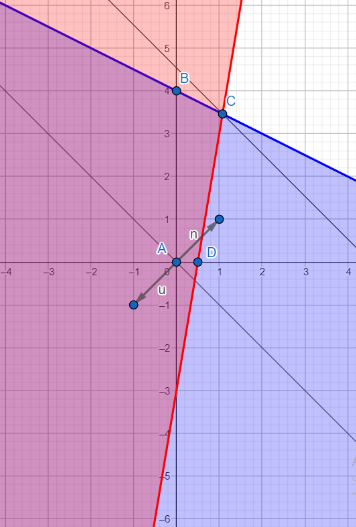
\includegraphics[]{пункт а.png}
\centering
\caption{График для решения задания №1, пункта 1a (построен с помощью \url{https://www.geogebra.org/calculator})}
\end{figure}

Без учета требования целочисленности:\\
Область допустимых значений - четырехугольник ABCD\\
$F_{max} = F(\frac{14}{13}; \frac{45}{13}) = \frac{59}{13}$
$x_1, x_2$ нецелочисленные\\

\begin{flushleft}
    {\bf2. Решение задачи симплекс методом} - см. №2а\\
\end{flushleft}

\begin{flushleft}
Приведем задачу к канонической форме:
\end{flushleft}

\begin{equation*}
    \begin{cases}
        x_1 + 2x_2 + x_3 = 8 \\
        6x_1 - x_2 + x_4 = 3 \\
        x_1, x_2 \in N_0, x_3, x_4 \ge 0
    \end{cases}
\end{equation*}

Оптимальная симплекс таблица без учета требования целочисленности:

\begin{center}
    \begin{tabular}{|c | c c c c c|} 
         \hline
            Базис & $x_1$ & $x_2$ & $x_3$ & $x_4$ & $b_i$\\
         \hline
            $x_2$ & 0 & 2 & $\frac{12}{13}$ & $-\frac{2}{13}$ & $\frac{90}{13}$\\
         \hline
            $x_1$ & 6.5 & 0 & 0.5 & 1 & 7\\
         \hline
            F(x) & 0 & 0 & $\frac{7}{13}$ & 1 & $\frac{59}{13}$\\
         \hline
    \end{tabular}
\end{center}

\begin{center}
    \begin{tabular}{|c | c c c c c|} 
         \hline
            Базис & $x_1$ & $x_2$ & $x_3$ & $x_4$ & $b_i$\\
         \hline
            $x_2$ & 0 & 1 & $\frac{6}{13}$ & $-\frac{1}{13}$ & $\frac{45}{13}$\\
         \hline
            $x_1$ & 1 & 0 & $\frac{1}{13}$ & $\frac{2}{13}$ & $\frac{14}{13}$\\
         \hline
            F(x) & 0 & 0 & $\frac{7}{13}$ & 1 & $\frac{59}{13}$\\
         \hline
    \end{tabular}
\end{center}

$F_{max} = F(\frac{14}{13}; \frac{45}{13}) = \frac{59}{13}$\\
$x_1, x_2$ нецелочисленные\\

\begin{flushleft}
    {\bf3. Решение задачи методом отсечения Гомори}\\
    {\bf3.1. Геометрическим методом}\\
\end{flushleft}

\begin{figure}[ht]
\centering
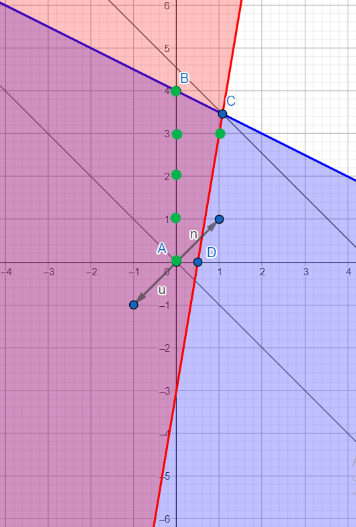
\includegraphics[]{пункт а_1.png}
\centering
\caption{График для решения ЗЦЛП (построен с помощью \url{https://www.geogebra.org/calculator})}
\end{figure}
Допустимые значения - множество зеленых точек\\
$\vec{n}\{1; 1\}$ - $\nabla F$ (градиент)\\
Если перемещать линию уровня (перпендикулярна $\vec{n}$) в направлении $\vec{n}$, то последняя точка, через которую пройдет линия, - точка с координатами (1; 3) - оптимальная точка\\
Значит $F_{max} = F(1; 3) = 1 + 3 = 4$\\
{\bfОтвет:~} $F_{max} = F(1; 3) = 4$

\begin{flushleft}
    {\bf3.2. Симплекс методом}\\
\end{flushleft}

Т.к. $\{\frac{45}{13}\} > \{\frac{14}{13}\}$, выпишем неравенство, соответствующее строке для $x_2$ в оптимальной симплекс таблице нецелочисленной задачи:\\
$\{0\} \cdot x_1 + \{1\} \cdot x_2 + \frac{6}{13} \cdot x_3 -\frac{1}{13} \cdot x_4 \ge \{\frac{45}{13}\}$\\
$\frac{6}{13} \cdot x_3 - \frac{1}{13} \cdot x_4 \ge \frac{6}{13}$\\
\begin{equation*}
    \begin{cases}
        6x_3 - x_4 \ge 6 \\
        x_3 = 8 - x_1 - 2x_2\\
        x_4 = 3 - 6x_1 + x_2\\
    \end{cases}
\end{equation*}
Значит:\\
$6\cdot (8 - x_1 - 2x_2) - (3 - 6x_1 + x_2) \ge 6$\\
$48 - 6x_1 - 12x_2 - 3 + 6x_1 - x_2 \ge 6$\\
$45 - 13x_2 \ge 6$\\
$x_1 \le 3$\\

Новая система ограничений:
\begin{equation*}
    \begin{cases}
        x_1 + 2x_2 \le 8 \\
        6x_1 - x_2 \le 3 \\
        x_2 \le 3\\
        x_1, x_2 \in N_0 
    \end{cases}
\end{equation*}

Каноническая форма:
\begin{equation*}
    \begin{cases}
        x_1 + 2x_2 + x_3 = 8 \\
        6x_1 - x_2 + x_4 = 3 \\
        x_2 + x_5 = 3\\
        x_1, x_2 \in N_0, x_3, x_4, x_5 \ge 0 
    \end{cases}
\end{equation*}

{\bf1-я симплекс-таблица:}

\begin{center}
    \begin{tabular}{|c | g c c c c c c|} 
         \hline
            Базис & $x_1$ & $x_2$ & $x_3$ & $x_4$ & $x_5$ & $b_i$ & $b_i/$р.с.\\
         \hline
            $x_3$ & 1 & 2 & 1 & 0 & 0 & 8 & 8/1 = 8\\
         \hline
         \rowcolor{LightBlue}
            $x_4$ & \cellcolor{cyan}6 & -1 & 0 & 1 & 0 & 3 & 3/6 = 1/2\\
         \hline
            $x_5$ & 0 & 1 & 0 & 0 & 1 & 3 & - \\
         \hline
            F(x) & -1 & -1 & 0 & 0 & 0 & 0 &\\
         \hline
    \end{tabular}
\end{center}

\begin{flushleft}
    Наименьшее значение в строке F(x): -1\\
    Разрешающий столбец: $x_1$\\
    Минимальное положительное значение из столбца $b_i$/р.с. : 1/2\\
    Разрешающий элемент: 6\\
    Не все значения в строке F(x) положительные $\implies$ решение не оптимально, строим новую таблицу\\
    {\bf2-я симплекс-таблица:}\\
\end{flushleft}

\begin{center}
    \begin{tabular}{|c | c g c c c c c|} 
         \hline
            Базис & $x_1$ & $x_2$ & $x_3$ & $x_4$ & $x_5$ & $b_i$ & $b_i/$р.с.\\
         \hline
            $x_3$ & 0 & $\frac{13}{6}$ & 1 & $-\frac{1}{6}$ & 0 & 7.5 & 7.5/($\frac{13}{6}$) = $\frac{45}{13}$\\
         \hline
            $x_1$ & 6 & -1 & 0 & 1 & 0 & 3 & 3/(-1) = -3\\
         \hline
         \rowcolor{LightBlue}
            $x_5$ & 0 & \cellcolor{cyan}1 & 0 & 0 & 1 & 3 & 3/1 = 3 \\
         \hline
            F(x) & 0 & $-\frac{7}{6}$ & 0 & $\frac{1}{6}$ & 0 & 0.5 &\\
         \hline
    \end{tabular}
\end{center}

\begin{flushleft}
    Наименьшее значение в строке F(x): $-\frac{7}{6}$\\
    Разрешающий столбец: $x_2$\\
    Минимальное положительное значение из столбца $b_i$/р.с. : 3\\
    Разрешающий элемент: $\frac{1}{6}$\\
    Не все значения в строке F(x) положительные $\implies$ решение не оптимально, строим новую таблицу\\
    {\bf3-я симплекс-таблица:}\\
\end{flushleft}

\begin{center}
    \begin{tabular}{|c | c c c c c c c|} 
         \hline
            Базис & $x_1$ & $x_2$ & $x_3$ & $x_4$ & $x_5$ & $b_i$ & $b_i/$р.с.\\
         \hline
            $x_3$ & 0 & 0 & 1 & $-\frac{1}{6}$ & $-\frac{13}{6}$ & 1 & \\
         \hline
            $x_1$ & 6 & 0 & 0 & 1 & 1 & 6 & \\
         \hline
            $x_2$ & 0 & 1 & 0 & 0 & 1 & 3 & \\
         \hline
            F(x) & 0 & 0 & 0 & $\frac{1}{6}$ & $\frac{7}{6}$ & 4 &\\
         \hline
    \end{tabular}
\end{center}

\begin{flushleft}
    Все значения в строке F(x) положительные, $F_{max} = 4$\\
    Оптимальное решение:\\
    $x_1 = 6/6 = 1$\\
    $x_2 = 3/1 = 3$\\
    $x_1, x_2$ целые $\implies$ задача целочисленного линейного программирования решена
\end{flushleft}

{\bfОтвет:~} $F_{max} = F(1; 3) = 4$

\chapter{Задача коммивояжера}

Решить задачу коммивояжера с 10 городами.

\begin{center}
    \begin{tabular}{|a | c | c | c | c | c | c | c | c | c | c|} 
         \hline
         \rowcolor{LightGray}
            & 1 & 2 & 3 & 4 & 5 & 6 & 7 & 8 & 9 & 10\\
         \hline
            1 & \cellcolor{Beige}$\infty$ & 13 & 16 & 44 & 27 & 71 & 38 & 62 & 83 & 33\\
         \hline
            2 & 31 & \cellcolor{Beige}$\infty$ & 43 & 96 & 18 & 83 & 25 & 79 & 12 & 22\\
         \hline
            3 & 18 & 12 & \cellcolor{Beige}$\infty$ & 89 & 33 & 26 & 41 & 37 & 77 & 94\\
         \hline
            4 & 63 & 46 & 71 & \cellcolor{Beige}$\infty$ & 92 & 47 & 59 & 84 & 32 & 15\\
        \hline
            5 & 23 & 57 & 79 & 34 & \cellcolor{Beige}$\infty$ & 42 & 83 & 79 & 95 & 42\\
         \hline
            6 & 57 & 11 & 28 & 65 & 34 & \cellcolor{Beige}$\infty$ & 40 & 74 & 39 & 53\\
         \hline
            7 & 96 & 38 & 50 & 29 & 82 & 49 & \cellcolor{Beige}$\infty$ & 51 & 22 & 19\\
         \hline
            8 & 66 & 48 & 72 & 58 & 93 & 41 & 54 & \cellcolor{Beige}$\infty$ & 70 & 53\\
        \hline
            9 & 73 & 13 & 56 & 89 & 31 & 23 & 45 & 30 & \cellcolor{Beige}$\infty$ & 92\\
         \hline
            10 & 60 & 47 & 77 & 55 & 99 & 44 & 55 & 38 & 16 & \cellcolor{Beige}$\infty$\\
        \hline
    \end{tabular}
\end{center}

\begin{center}
    {\bf
    Решение:}
\end{center}

\begin{center}
    \begin{tabular}{|a | c | c | c | c | c | c | c | c | c | c | g|} 
         \hline
         \rowcolor{LightGray}
            & 1 & 2 & 3 & 4 & 5 & 6 & 7 & 8 & 9 & 10 & min\\
         \hline
            1 & \cellcolor{Beige}$\infty$ & 13 & 16 & 44 & 27 & 71 & 38 & 62 & 83 & 33 & 13\\
         \hline
            2 & 31 & \cellcolor{Beige}$\infty$ & 43 & 96 & 18 & 83 & 25 & 79 & 12 & 22 & 12\\
         \hline
            3 & 18 & 12 & \cellcolor{Beige}$\infty$ & 89 & 33 & 26 & 41 & 37 & 77 & 94 & 12\\
         \hline
            4 & 63 & 46 & 71 & \cellcolor{Beige}$\infty$ & 92 & 47 & 59 & 84 & 32 & 15 & 15\\
        \hline
            5 & 23 & 57 & 79 & 34 & \cellcolor{Beige}$\infty$ & 42 & 83 & 79 & 95 & 42 & 23\\
         \hline
            6 & 57 & 11 & 28 & 65 & 34 & \cellcolor{Beige}$\infty$ & 40 & 74 & 39 & 53 & 11\\
         \hline
            7 & 96 & 38 & 50 & 29 & 82 & 49 & \cellcolor{Beige}$\infty$ & 51 & 22 & 19 & 19\\
         \hline
            8 & 66 & 48 & 72 & 58 & 93 & 41 & 54 & \cellcolor{Beige}$\infty$ & 70 & 53 & 41\\
        \hline
            9 & 73 & 13 & 56 & 89 & 31 & 23 & 45 & 30 & \cellcolor{Beige}$\infty$ & 92 & 13\\
         \hline
            10 & 60 & 47 & 77 & 55 & 99 & 44 & 55 & 38 & 16 & \cellcolor{Beige}$\infty$ & 16\\
        \hline
    \end{tabular}
\end{center}

\begin{center}
    \begin{tabular}{|a | c | c | c | c | c | c | c | c | c | c|} 
         \hline
         \rowcolor{LightGray}
            & 1 & 2 & 3 & 4 & 5 & 6 & 7 & 8 & 9 & 10\\
         \hline
            1 & \cellcolor{Beige}$\infty$ & 0 & 3 & 31 & 14 & 58 & 25 & 49 & 70 & 20\\
         \hline
            2 & 19 & \cellcolor{Beige}$\infty$ & 31 & 84 & 6 & 71 & 13 & 67 & 0 & 10\\
         \hline
            3 & 6 & 0 & \cellcolor{Beige}$\infty$ & 77 & 21 & 14 & 29 & 25 & 65 & 82\\
         \hline
            4 & 48 & 31 & 56 & \cellcolor{Beige}$\infty$ & 77 & 32 & 44 & 69 & 17 & 0\\
        \hline
            5 & 0 & 34 & 56 & 11 & \cellcolor{Beige}$\infty$ & 19 & 60 & 56 & 72 & 19\\
         \hline
            6 & 46 & 0 & 17 & 54 & 23 & \cellcolor{Beige}$\infty$ & 29 & 63 & 28 & 42\\
         \hline
            7 & 77 & 19 & 31 & 10 & 63 & 30 & \cellcolor{Beige}$\infty$ & 32 & 3 & 0\\
         \hline
            8 & 25 & 7 & 31 & 17 & 52 & 0 & 13 & \cellcolor{Beige}$\infty$ & 29 & 12\\
        \hline
            9 & 60 & 0 & 43 & 76 & 18 & 10 & 32 & 17 & \cellcolor{Beige}$\infty$ & 79\\
         \hline
            10 & 44 & 31 & 61 & 39 & 83 & 28 & 39 & 22 & 0 & \cellcolor{Beige}$\infty$\\
        \hline
        \rowcolor{LightBlue}
            min & 0 & 0 & 3 & 10 & 6 & 0 & 13 & 17 & 0 & 0\\
         \hline
    \end{tabular}
\end{center}

Нижняя граница издержек - сумма приводящих констант:\\
$h = (13 + 12 + 12 + 15 + 23 + 11 + 19 + 41 + 13 + 16) + (3 + 10 + 6 + 13 + 17) = 224$\\
$G_0$ - множество всех маршрутов\\
$w(G_0) = h = 224$

\begin{center}
    \begin{tabular}{|a | c | c | c | c | c | c | c | c | c | c | g|} 
         \hline
         \rowcolor{LightGray}
            & 1 & 2 & 3 & 4 & 5 & 6 & 7 & 8 & 9 & 10 & \\
         \hline
            1 & \cellcolor{Beige}$\infty$ & 0 & 0 & 21 & 8 & 58 & 12 & 32 & 70 & 20 & 0\\
         \hline
            2 & 19 & \cellcolor{Beige}$\infty$ & 28 & 74 & 0 & 71 & 0 & 50 & 0 & 10 & 0\\
         \hline
            3 & 6 & 0 & \cellcolor{Beige}$\infty$ & 67 & 15 & 14 & 16 & 8 & 65 & 82 & 6\\
         \hline
            4 & 48 & 31 & 53 & \cellcolor{Beige}$\infty$ & 71 & 32 & 31 & 52 & 17 & 0 & 17\\
        \hline
            5 & 0 & 34 & 53 & 1 & \cellcolor{Beige}$\infty$ & 19 & 47 & 39 & 72 & 19 & 1\\
         \hline
            6 & 46 & 0 & 14 & 44 & 17 & \cellcolor{Beige}$\infty$ & 16 & 46 & 28 & 42 & 14\\
         \hline
            7 & 77 & 19 & 28 & 0 & 57 & 30 & \cellcolor{Beige}$\infty$ & 15 & 3 & 0 & 0\\
         \hline
            8 & 25 & 7 & 28 & 7 & 46 & 0 & 0 & \cellcolor{Beige}$\infty$ & 29 & 12 & 0\\
        \hline
            9 & 60 & 0 & 40 & 66 & 12 & 10 & 19 & 0 & \cellcolor{Beige}$\infty$ & 79 & 0\\
         \hline
            10 & 44 & 31 & 58 & 29 & 77 & 28 & 26 & 5 & 0 & \cellcolor{Beige}$\infty$ & 5\\
        \hline
        \rowcolor{LightBlue}
             & 6 & 0 & 14 & 1 & 8 & 10 & 0 & 5 & 0 & 0 &\\
         \hline
    \end{tabular}
\end{center}

Претенденты на ветвление:\\
$S_{12}, S_{13}, S_{25}, S_{27}, S_{29}, S_{32}, S_{4,10}, S_{51}, S_{62}, S_{74}, S_{7,10}, S_{86}, S_{87}, S_{92}, S_{98}, S_{10,9} = 0$\\
$Q_{12} = 0 + 0 = 0$\\
$Q_{13} = 14 + 0 = 0$\\
$Q_{25} = 8 + 0 = 8$\\
$Q_{27} = 0 + 0 = 0$\\
$Q_{29} = 0 + 0 = 0$\\
$Q_{32} = 0 + 6 = 6$\\
$Q_{4,10} = 0 + 17 = 17$\\
$Q_{51} = 0 + 1 = 1$\\
$Q_{62} = 0 + 14 = 14$\\
$Q_{74} = 1 + 0 = 1$\\
$Q_{7,10} = 0 + 0 = 0$\\
$Q_{86} = 10 + 0 = 10$\\
$Q_{87} = 0 + 0 = 0$\\
$Q_{92} = 0 + 0 = 0$\\
$Q_{98} = 5 + 0 = 5$\\
$Q_{10,9} = 0 + 5 = 5$\\

$Q_{max} = Q_{4,10} = 17 \implies$ выбираем для ветвления пару (4, 10)\\
$w(\overline{\{4, 10\}}) = 224 + 17 = 241$

\begin{center}
    \begin{tabular}{|a | c | c | c | c | c | c | c | c | c |} 
         \hline
         \rowcolor{LightGray}
            & 1 & 2 & 3 & 4 & 5 & 6 & 7 & 8 & 9 \\
         \hline
            1 & \cellcolor{Beige}$\infty$ & 0 & 0 & 21 & 8 & 58 & 12 & 32 & 70 \\
         \hline
            2 & 19 & \cellcolor{Beige}$\infty$ & 28 & 74 & 0 & 71 & 0 & 50 & 0 \\
         \hline
            3 & 6 & 0 & \cellcolor{Beige}$\infty$ & 67 & 15 & 14 & 16 & 8 & 65 \\
         \hline
            5 & 0 & 34 & 53 & 1 & \cellcolor{Beige}$\infty$ & 19 & 47 & 39 & 72 \\
         \hline
            6 & 46 & 0 & 14 & 44 & 17 & \cellcolor{Beige}$\infty$ & 16 & 46 & 28 \\
         \hline
            7 & 77 & 19 & 28 & 0 & 57 & 30 & \cellcolor{Beige}$\infty$ & 15 & 3 \\
         \hline
            8 & 25 & 7 & 28 & 7 & 46 & 0 & 0 & \cellcolor{Beige}$\infty$ & 29 \\
        \hline
            9 & 60 & 0 & 40 & 66 & 12 & 10 & 19 & 0 & \cellcolor{Beige}$\infty$ \\
         \hline
            10 & 44 & 31 & 58 & \cellcolor{Beige}$\infty$ & 77 & 28 & 26 & 5 & 0\\
        \hline
    \end{tabular}
\end{center}

\begin{center}
    \begin{tabular}{|a | c | c | c | c | c | c | c | c | c | g|} 
         \hline
         \rowcolor{LightGray}
            & 1 & 2 & 3 & 4 & 5 & 6 & 7 & 8 & 9 & min \\
         \hline
            1 & \cellcolor{Beige}$\infty$ & 0 & 0 & 21 & 8 & 58 & 12 & 32 & 70 & 0\\
         \hline
            2 & 19 & \cellcolor{Beige}$\infty$ & 28 & 74 & 0 & 71 & 0 & 50 & 0 & 0\\
         \hline
            3 & 6 & 0 & \cellcolor{Beige}$\infty$ & 67 & 15 & 14 & 16 & 8 & 65 & 0 \\
         \hline
            5 & 0 & 34 & 53 & 1 & \cellcolor{Beige}$\infty$ & 19 & 47 & 39 & 72 & 0 \\
         \hline
            6 & 46 & 0 & 14 & 44 & 17 & \cellcolor{Beige}$\infty$ & 16 & 46 & 28 & 0\\
         \hline
            7 & 77 & 19 & 28 & 0 & 57 & 30 & \cellcolor{Beige}$\infty$ & 15 & 3 & 0 \\
         \hline
            8 & 25 & 7 & 28 & 7 & 46 & 0 & 0 & \cellcolor{Beige}$\infty$ & 29 & 0 \\
        \hline
            9 & 60 & 0 & 40 & 66 & 12 & 10 & 19 & 0 & \cellcolor{Beige}$\infty$ & 0 \\
         \hline
            10 & 44 & 31 & 58 & \cellcolor{Beige}$\infty$ & 77 & 28 & 26 & 5 & 0 & 0\\
        \hline
    \end{tabular}
\end{center}

\begin{center}
    \begin{tabular}{|a | c | c | c | c | c | c | c | c | c |} 
         \hline
         \rowcolor{LightGray}
            & 1 & 2 & 3 & 4 & 5 & 6 & 7 & 8 & 9 \\
         \hline
            1 & \cellcolor{Beige}$\infty$ & 0 & 0 & 21 & 8 & 58 & 12 & 32 & 70 \\
         \hline
            2 & 19 & \cellcolor{Beige}$\infty$ & 28 & 74 & 0 & 71 & 0 & 50 & 0 \\
         \hline
            3 & 6 & 0 & \cellcolor{Beige}$\infty$ & 67 & 15 & 14 & 16 & 8 & 65 \\
         \hline
            5 & 0 & 34 & 53 & 1 & \cellcolor{Beige}$\infty$ & 19 & 47 & 39 & 72 \\
         \hline
            6 & 46 & 0 & 14 & 44 & 17 & \cellcolor{Beige}$\infty$ & 16 & 46 & 28 \\
         \hline
            7 & 77 & 19 & 28 & 0 & 57 & 30 & \cellcolor{Beige}$\infty$ & 15 & 3 \\
         \hline
            8 & 25 & 7 & 28 & 7 & 46 & 0 & 0 & \cellcolor{Beige}$\infty$ & 29 \\
        \hline
            9 & 60 & 0 & 40 & 66 & 12 & 10 & 19 & 0 & \cellcolor{Beige}$\infty$ \\
         \hline
            10 & 44 & 31 & 58 & \cellcolor{Beige}$\infty$ & 77 & 28 & 26 & 5 & 0\\
        \hline
        \rowcolor{LightBlue}
             min & 0 & 0 & 0 & 0 & 0 & 0 & 0 & 0 & 0\\
         \hline
    \end{tabular}
\end{center}

Сумма приводящих констант: $h = 0 + 0 = 0$\\
$w(\{4, 10\}) = 224 + 0 = 224 < 241 \implies$ включаем (4, 10) в маршрут

\begin{center}
    \begin{tabular}{|a | c | c | c | c | c | c | c | c | c | g|} 
         \hline
         \rowcolor{LightGray}
            & 1 & 2 & 3 & 4 & 5 & 6 & 7 & 8 & 9 &  \\
         \hline
            1 & \cellcolor{Beige}$\infty$ & 0 & 0 & 21 & 8 & 58 & 12 & 32 & 70 & 0\\
         \hline
            2 & 19 & \cellcolor{Beige}$\infty$ & 28 & 74 & 0 & 71 & 0 & 50 & 0 & 0\\
         \hline
            3 & 6 & 0 & \cellcolor{Beige}$\infty$ & 67 & 15 & 14 & 16 & 8 & 65 & 6 \\
         \hline
            5 & 0 & 34 & 53 & 1 & \cellcolor{Beige}$\infty$ & 19 & 47 & 39 & 72 & 1 \\
         \hline
            6 & 46 & 0 & 14 & 44 & 17 & \cellcolor{Beige}$\infty$ & 16 & 46 & 28 & 14\\
         \hline
            7 & 77 & 19 & 28 & 0 & 57 & 30 & \cellcolor{Beige}$\infty$ & 15 & 3 & 3 \\
         \hline
            8 & 25 & 7 & 28 & 7 & 46 & 0 & 0 & \cellcolor{Beige}$\infty$ & 29 & 0 \\
        \hline
            9 & 60 & 0 & 40 & 66 & 12 & 10 & 19 & 0 & \cellcolor{Beige}$\infty$ & 0 \\
         \hline
            10 & 44 & 31 & 58 & \cellcolor{Beige}$\infty$ & 77 & 28 & 26 & 5 & 0 & 5\\
        \hline
        \rowcolor{LightBlue}
              & 6 & 0 & 14 & 1 & 8 & 10 & 0 & 5 & 0 & \\
         \hline
    \end{tabular}
\end{center}

Претенденты на ветвление:\\
$S_{12}, S_{13}, S_{25}, S_{27}, S_{29}, S_{32}, S_{51}, S_{62}, S_{74}, S_{86}, S_{87}, S_{92}, S_{98}, S_{10,9} = 0$\\
$Q_{12} = 0 + 0 = 0$\\
$Q_{13} = 14 + 0 = 14$\\
$Q_{25} = 8 + 0 = 8$\\
$Q_{27} = 0 + 0 = 0$\\
$Q_{29} = 0 + 0 = 0$\\
$Q_{32} = 0 + 6 = 6$\\
$Q_{51} = 6 + 1 = 7$\\
$Q_{62} = 0 + 14 = 14$\\
$Q_{74} = 1 + 3 = 4$\\
$Q_{86} = 10 + 0 = 10$\\
$Q_{87} = 0 + 0 = 0$\\
$Q_{92} = 0 + 0 = 0$\\
$Q_{98} = 5 + 0 = 5$\\
$Q_{10,9} = 0 + 5 = 5$\\

$Q_{max} = Q_{13} = 14 \implies$ выбираем для ветвления пару (1, 3)\\
$w({\overline{\{1, 3\}}}) = w(\{4, 10\}) + Q_{max} = 224 + 14 = 238$

\begin{center}
    \begin{tabular}{|a | c | c | c | c | c | c | c | c|} 
         \hline
         \rowcolor{LightGray}
            & 1 & 2 & 4 & 5 & 6 & 7 & 8 & 9 \\
         \hline
            2 & 19 & \cellcolor{Beige}$\infty$ & 74 & 0 & 71 & 0 & 50 & 0 \\
         \hline
            3 & \cellcolor{Beige}$\infty$ & 0 & 67 & 15 & 14 & 16 & 8 & 65  \\
         \hline
            5 & 0 & 34 & 1 & \cellcolor{Beige}$\infty$ & 19 & 47 & 39 & 72  \\
         \hline
            6 & 46 & 0 & 44 & 17 & \cellcolor{Beige}$\infty$ & 16 & 46 & 28 \\
         \hline
            7 & 77 & 19 & 0 & 57 & 30 & \cellcolor{Beige}$\infty$ & 15 & 3 \\
         \hline
            8 & 25 & 7 & 7 & 46 & 0 & 0 & \cellcolor{Beige}$\infty$ & 29 \\
        \hline
            9 & 60 & 0 & 66 & 12 & 10 & 19 & 0 & \cellcolor{Beige}$\infty$ \\
         \hline
            10 & 44 & 31 & \cellcolor{Beige}$\infty$ & 77 & 28 & 26 & 5 & 0 \\
        \hline
    \end{tabular}
\end{center}

\begin{center}
    \begin{tabular}{|a | c | c | c | c | c | c | c | c | g|} 
         \hline
         \rowcolor{LightGray}
            & 1 & 2 & 4 & 5 & 6 & 7 & 8 & 9 & min\\
         \hline
            2 & 19 & \cellcolor{Beige}$\infty$ & 74 & 0 & 71 & 0 & 50 & 0 & 0\\
         \hline
            3 & \cellcolor{Beige}$\infty$ & 0 & 67 & 15 & 14 & 16 & 8 & 65 & 0 \\
         \hline
            5 & 0 & 34 & 1 & \cellcolor{Beige}$\infty$ & 19 & 47 & 39 & 72 & 0 \\
         \hline
            6 & 46 & 0 & 44 & 17 & \cellcolor{Beige}$\infty$ & 16 & 46 & 28 & 0  \\
         \hline
            7 & 77 & 19 & 0 & 57 & 30 & \cellcolor{Beige}$\infty$ & 15 & 3 & 0 \\
         \hline
            8 & 25 & 7 & 7 & 46 & 0 & 0 & \cellcolor{Beige}$\infty$ & 29 & 0 \\
        \hline
            9 & 60 & 0 & 66 & 12 & 10 & 19 & 0 & \cellcolor{Beige}$\infty$ & 0 \\
         \hline
            10 & 44 & 31 & \cellcolor{Beige}$\infty$ & 77 & 28 & 26 & 5 & 0 & 0 \\
        \hline
    \end{tabular}
\end{center}

\begin{center}
    \begin{tabular}{|a | c | c | c | c | c | c | c | c|} 
         \hline
         \rowcolor{LightGray}
            & 1 & 2 & 4 & 5 & 6 & 7 & 8 & 9 \\
         \hline
            2 & 19 & \cellcolor{Beige}$\infty$ & 74 & 0 & 71 & 0 & 50 & 0 \\
         \hline
            3 & \cellcolor{Beige}$\infty$ & 0 & 67 & 15 & 14 & 16 & 8 & 65  \\
         \hline
            5 & 0 & 34 & 1 & \cellcolor{Beige}$\infty$ & 19 & 47 & 39 & 72  \\
         \hline
            6 & 46 & 0 & 44 & 17 & \cellcolor{Beige}$\infty$ & 16 & 46 & 28 \\
         \hline
            7 & 77 & 19 & 0 & 57 & 30 & \cellcolor{Beige}$\infty$ & 15 & 3 \\
         \hline
            8 & 25 & 7 & 7 & 46 & 0 & 0 & \cellcolor{Beige}$\infty$ & 29 \\
        \hline
            9 & 60 & 0 & 66 & 12 & 10 & 19 & 0 & \cellcolor{Beige}$\infty$ \\
         \hline
            10 & 44 & 31 & \cellcolor{Beige}$\infty$ & 77 & 28 & 26 & 5 & 0 \\
        \hline
        \rowcolor{LightBlue}
              min & 0 & 0 & 0 & 0 & 0 & 0 & 0 & 0 \\
         \hline
    \end{tabular}
\end{center}

Сумма приводящих констант: $h = 0 + 0 = 0$\\
$w(\{1, 3\}) = w(\{4, 10\}) + h = 224 + 0 = 224 < 238 \implies$ включаем (1, 3) в маршрут

\begin{center}
    \begin{tabular}{|a | c | c | c | c | c | c | c | c | g|} 
         \hline
         \rowcolor{LightGray}
            & 1 & 2 & 4 & 5 & 6 & 7 & 8 & 9 & \\
         \hline
            2 & 19 & \cellcolor{Beige}$\infty$ & 74 & 0 & 71 & 0 & 50 & 0 & 0 \\
         \hline
            3 & \cellcolor{Beige}$\infty$ & 0 & 67 & 15 & 14 & 16 & 8 & 65 & 8 \\
         \hline
            5 & 0 & 34 & 1 & \cellcolor{Beige}$\infty$ & 19 & 47 & 39 & 72 & 1 \\
         \hline
            6 & 46 & 0 & 44 & 17 & \cellcolor{Beige}$\infty$ & 16 & 46 & 28 & 16 \\
         \hline
            7 & 77 & 19 & 0 & 57 & 30 & \cellcolor{Beige}$\infty$ & 15 & 3 & 3 \\
         \hline
            8 & 25 & 7 & 7 & 46 & 0 & 0 & \cellcolor{Beige}$\infty$ & 29 & 0 \\
        \hline
            9 & 60 & 0 & 66 & 12 & 10 & 19 & 0 & \cellcolor{Beige}$\infty$ & 0\\
         \hline
            10 & 44 & 31 & \cellcolor{Beige}$\infty$ & 77 & 28 & 26 & 5 & 0 & 5\\
        \hline
        \rowcolor{LightBlue}
               & 19 & 0 & 1 & 12 & 10 & 0 & 5 & 0 & \\
         \hline
    \end{tabular}
\end{center}

Претенденты на ветвление:\\
$S_{25}, S_{27}, S_{29}, S_{32}, S_{51}, S_{62}, S_{74}, S_{86}, S_{87}, S_{92}, S_{98}, S_{10,9} = 0$\\
$Q_{25} = 12 + 0 = 12$\\
$Q_{27} = 0 + 0 = 0$\\
$Q_{29} = 0 + 0 = 0$\\
$Q_{32} = 0 + 8 = 8$\\
$Q_{51} = 19 + 1 = 20$\\
$Q_{62} = 0 + 16 = 16$\\
$Q_{74} = 1 + 3 = 4$\\
$Q_{86} = 10 + 0 = 10$\\
$Q_{87} = 0 + 0 = 0$\\
$Q_{92} = 0 + 0 = 0$\\
$Q_{98} = 5 + 0 = 5$\\
$Q_{10,9} = 0 + 5 = 5$\\

$Q_{max} = Q_{51} = 20 \implies$ выбираем для ветвления пару (5, 1)\\
$w(\{\overline{5, 1}\}) = w(\{1, 3\}) + G_{max} = 224 + 20 = 244$

Запрещаем переход (3, 5), так как в маршруте есть пары (1, 3) и (5, 1)

\begin{center}
    \begin{tabular}{|a | c | c | c | c | c | c | c | c|} 
         \hline
         \rowcolor{LightGray}
            & 2 & 4 & 5 & 6 & 7 & 8 & 9 \\
         \hline
            2 & \cellcolor{Beige}$\infty$ & 74 & 0 & 71 & 0 & 50 & 0 \\
         \hline
            3 & 0 & 67 & \cellcolor{Beige}$\infty$ & 14 & 16 & 8 & 65 \\
         \hline
            6 & 0 & 44 & 17 & \cellcolor{Beige}$\infty$ & 16 & 46 & 28 \\
         \hline
            7 & 19 & 0 & 57 & 30 & \cellcolor{Beige}$\infty$ & 15 & 3 \\
         \hline
            8 & 7 & 7 & 46 & 0 & 0 & \cellcolor{Beige}$\infty$ & 29 \\
        \hline
            9 & 0 & 66 & 12 & 10 & 19 & 0 & \cellcolor{Beige}$\infty$\\
         \hline
            10 & 31 & \cellcolor{Beige}$\infty$ & 77 & 28 & 26 & 5 & 0\\
        \hline
    \end{tabular}
\end{center}

\begin{center}
    \begin{tabular}{|a | c | c | c | c | c | c | c | g|} 
         \hline
         \rowcolor{LightGray}
            & 2 & 4 & 5 & 6 & 7 & 8 & 9 & min \\
         \hline
            2 & \cellcolor{Beige}$\infty$ & 74 & 0 & 71 & 0 & 50 & 0 & 0\\
         \hline
            3 & 0 & 67 & \cellcolor{Beige}$\infty$ & 14 & 16 & 8 & 65 & 0 \\
         \hline
            6 & 0 & 44 & 17 & \cellcolor{Beige}$\infty$ & 16 & 46 & 28 & 0 \\
         \hline
            7 & 19 & 0 & 57 & 30 & \cellcolor{Beige}$\infty$ & 15 & 3 & 0 \\
         \hline
            8 & 7 & 7 & 46 & 0 & 0 & \cellcolor{Beige}$\infty$ & 29 & 0 \\
        \hline
            9 & 0 & 66 & 12 & 10 & 19 & 0 & \cellcolor{Beige}$\infty$ & 0\\
         \hline
            10 & 31 & \cellcolor{Beige}$\infty$ & 77 & 28 & 26 & 5 & 0 & 0\\
        \hline
    \end{tabular}
\end{center}

\begin{center}
    \begin{tabular}{|a | c | c | c | c | c | c | c | c|} 
         \hline
         \rowcolor{LightGray}
            & 2 & 4 & 5 & 6 & 7 & 8 & 9 \\
         \hline
            2 & \cellcolor{Beige}$\infty$ & 74 & 0 & 71 & 0 & 50 & 0 \\
         \hline
            3 & 0 & 67 & \cellcolor{Beige}$\infty$ & 14 & 16 & 8 & 65 \\
         \hline
            6 & 0 & 44 & 17 & \cellcolor{Beige}$\infty$ & 16 & 46 & 28 \\
         \hline
            7 & 19 & 0 & 57 & 30 & \cellcolor{Beige}$\infty$ & 15 & 3 \\
         \hline
            8 & 7 & 7 & 46 & 0 & 0 & \cellcolor{Beige}$\infty$ & 29 \\
        \hline
            9 & 0 & 66 & 12 & 10 & 19 & 0 & \cellcolor{Beige}$\infty$\\
         \hline
            10 & 31 & \cellcolor{Beige}$\infty$ & 77 & 28 & 26 & 5 & 0\\
        \hline
        \rowcolor{LightBlue}
               min & 0 & 0 & 0 & 0 & 0 & 0 & 0 \\
         \hline
    \end{tabular}
\end{center}

Сумма приводящих констант: $h = 0 + 0 = 0$\\
$w(\{5, 1\}) = w(\{1, 3\}) + h = 224 + 0 = 224 < 244 \implies$ включаем (5, 1) в маршрут

\begin{center}
    \begin{tabular}{|a | c | c | c | c | c | c | c | g|} 
         \hline
         \rowcolor{LightGray}
            & 2 & 4 & 5 & 6 & 7 & 8 & 9 & \\
         \hline
            2 & \cellcolor{Beige}$\infty$ & 74 & 0 & 71 & 0 & 50 & 0 & 0 \\
         \hline
            3 & 0 & 67 & \cellcolor{Beige}$\infty$ & 14 & 16 & 8 & 65 & 8 \\
         \hline
            6 & 0 & 44 & 17 & \cellcolor{Beige}$\infty$ & 16 & 46 & 28 & 16 \\
         \hline
            7 & 19 & 0 & 57 & 30 & \cellcolor{Beige}$\infty$ & 15 & 3 & 3 \\
         \hline
            8 & 7 & 7 & 46 & 0 & 0 & \cellcolor{Beige}$\infty$ & 29 & 0 \\
        \hline
            9 & 0 & 66 & 12 & 10 & 19 & 0 & \cellcolor{Beige}$\infty$ & 0 \\
         \hline
            10 & 31 & \cellcolor{Beige}$\infty$ & 77 & 28 & 26 & 5 & 0 & 5 \\
        \hline
        \rowcolor{LightBlue}
            & 0 & 7 & 12 & 10 & 0 & 5 & 0 &  \\
         \hline
    \end{tabular}
\end{center}

Претенденты на ветвление:\\
$S_{25}, S_{27}, S_{29}, S_{32}, S_{62}, S_{74}, S_{86}, S_{87}, S_{92}, S_{98}, S_{10,9} = 0$\\
$Q_{25} = 12 + 0 = 12$\\
$Q_{27} = 0 + 0 = 0$\\
$Q_{29} = 0 + 0 = 0$\\
$Q_{32} = 0 + 8 = 8$\\
$Q_{62} = 0 + 16 = 16$\\
$Q_{74} = 7 + 3 = 10$\\
$Q_{86} = 10 + 0 = 10$\\
$Q_{87} = 0 + 0 = 0$\\
$Q_{92} = 0 + 0 = 0$\\
$Q_{98} = 5 + 0 = 5$\\
$Q_{10,9} = 0 + 5 = 5$\\

$Q_{max} = Q_{62} = 16 \implies$ выбираем для ветвления пару (6, 2)\\
$w(\{\overline{6, 2}\}) = w(\{5, 1\}) + Q_{max} = 224 + 16 = 240$

\begin{center}
    \begin{tabular}{|a | c | c | c | c | c | c|} 
         \hline
         \rowcolor{LightGray}
            & 4 & 5 & 6 & 7 & 8 & 9 \\
         \hline
            2 & 74 & 0 & \cellcolor{Beige}$\infty$ & 0 & 50 & 0 \\
         \hline
            3 & 67 & \cellcolor{Beige}$\infty$ & 14 & 16 & 8 & 65 \\
         \hline
            7 & 0 & 57 & 30 & \cellcolor{Beige}$\infty$ & 15 & 3 \\
         \hline
            8 & 7 & 46 & 0 & 0 & \cellcolor{Beige}$\infty$ & 29 \\
        \hline
            9 & 66 & 12 & 10 & 19 & 0 & \cellcolor{Beige}$\infty$ \\
         \hline
            10 & \cellcolor{Beige}$\infty$ & 77 & 28 & 26 & 5 & 0 \\
        \hline
    \end{tabular}
\end{center}

\begin{center}
    \begin{tabular}{|a | c | c | c | c | c | c | g|} 
         \hline
         \rowcolor{LightGray}
            & 4 & 5 & 6 & 7 & 8 & 9 & min \\
         \hline
            2 & 74 & 0 & \cellcolor{Beige}$\infty$ & 0 & 50 & 0 & 0 \\
         \hline
            3 & 67 & \cellcolor{Beige}$\infty$ & 14 & 16 & 8 & 65 & 8\\
         \hline
            7 & 0 & 57 & 30 & \cellcolor{Beige}$\infty$ & 15 & 3 & 0 \\
         \hline
            8 & 7 & 46 & 0 & 0 & \cellcolor{Beige}$\infty$ & 29 & 0 \\
        \hline
            9 & 66 & 12 & 10 & 19 & 0 & \cellcolor{Beige}$\infty$ & 0 \\
         \hline
            10 & \cellcolor{Beige}$\infty$ & 77 & 28 & 26 & 5 & 0 & 0 \\
        \hline
    \end{tabular}
\end{center}

\begin{center}
    \begin{tabular}{|a | c | c | c | c | c | c|} 
         \hline
         \rowcolor{LightGray}
            & 4 & 5 & 6 & 7 & 8 & 9 \\
         \hline
            2 & 74 & 0 & \cellcolor{Beige}$\infty$ & 0 & 50 & 0 \\
         \hline
            3 & 59 & \cellcolor{Beige}$\infty$ & 6 & 8 & 0 & 57 \\
         \hline
            7 & 0 & 57 & 30 & \cellcolor{Beige}$\infty$ & 15 & 3 \\
         \hline
            8 & 7 & 46 & 0 & 0 & \cellcolor{Beige}$\infty$ & 29 \\
        \hline
            9 & 66 & 12 & 10 & 19 & 0 & \cellcolor{Beige}$\infty$ \\
         \hline
            10 & \cellcolor{Beige}$\infty$ & 77 & 28 & 26 & 5 & 0 \\
        \hline
        \rowcolor{LightBlue}
            min & 0 & 0 & 0 & 0 & 0 & 0 \\
         \hline
    \end{tabular}
\end{center}

Сумма приводящих констант: $h = 8 + 0 = 8$\\
$w(\{6, 2\}) = w(\{5, 1\}) + h = 224 + 8 = 232 < 240 \implies$ включаем (6, 2) в маршрут

\begin{center}
    \begin{tabular}{|a | c | c | c | c | c | c | g|} 
         \hline
         \rowcolor{LightGray}
            & 4 & 5 & 6 & 7 & 8 & 9 & \\
         \hline
            2 & 74 & 0 & \cellcolor{Beige}$\infty$ & 0 & 50 & 0 & 0 \\
         \hline
            3 & 59 & \cellcolor{Beige}$\infty$ & 6 & 8 & 0 & 57 & 6 \\
         \hline
            7 & 0 & 57 & 30 & \cellcolor{Beige}$\infty$ & 15 & 3 & 3 \\
         \hline
            8 & 7 & 46 & 0 & 0 & \cellcolor{Beige}$\infty$ & 29 & 0 \\
        \hline
            9 & 66 & 12 & 10 & 19 & 0 & \cellcolor{Beige}$\infty$ & 10 \\
         \hline
            10 & \cellcolor{Beige}$\infty$ & 77 & 28 & 26 & 5 & 0 & 5\\
        \hline
        \rowcolor{LightBlue}
            & 7 & 12 & 6 & 0 & 0 & 0 & \\
         \hline
    \end{tabular}
\end{center}

Претенденты на ветвление:\\
$S_{25}, S_{27}, S_{29}, S_{38}, S_{74}, S_{86}, S_{87}, S_{98}, S_{10,9} = 0$\\
$Q_{25} = 12 + 0 = 12$\\
$Q_{27} = 0 + 0 = 0$\\
$Q_{29} = 0 + 0 = 0$\\
$Q_{38} = 0 + 6 = 6$\\
$Q_{74} = 7 + 3 = 10$\\
$Q_{86} = 6 + 0 = 6$\\
$Q_{87} = 0 + 0 = 0$\\
$Q_{98} = 0 + 10 = 10$\\
$Q_{10,9} = 0 + 5 = 5$\\

$Q_{max} = Q_{25} = 12 \implies$ выбираем для ветвления пару (2, 5)\\
$w(\{\overline{2, 5}\}) = w(\{6, 2\}) + Q_{max} = 232 + 12 = 244$\\
Запрещаем переход (3, 6), так как в маршруте есть пары (6, 2), (2, 5), (5, 1), (1, 3)

\begin{center}
    \begin{tabular}{|a | c | c | c | c | c|} 
         \hline
         \rowcolor{LightGray}
            & 4 & 6 & 7 & 8 & 9\\
         \hline
            3 & 59 & \cellcolor{Beige}$\infty$ & 8 & 0 & 57\\
         \hline
            7 & 0 & 30 & \cellcolor{Beige}$\infty$ & 15 & 3\\
         \hline
            8 & 7 & 0 & 0 & \cellcolor{Beige}$\infty$ & 29\\
        \hline
            9 & 66 & 10 & 19 & 0 & \cellcolor{Beige}$\infty$\\
         \hline
            10 & \cellcolor{Beige}$\infty$ & 28 & 26 & 5 & 0\\
        \hline
    \end{tabular}
\end{center}

\begin{center}
    \begin{tabular}{|a | c | c | c | c | c | g|} 
         \hline
         \rowcolor{LightGray}
            & 4 & 6 & 7 & 8 & 9 & min\\
         \hline
            3 & 59 & \cellcolor{Beige}$\infty$ & 8 & 0 & 57 & 0\\
         \hline
            7 & 0 & 30 & \cellcolor{Beige}$\infty$ & 15 & 3 & 0\\
         \hline
            8 & 7 & 0 & 0 & \cellcolor{Beige}$\infty$ & 29 & 0\\
        \hline
            9 & 66 & 10 & 19 & 0 & \cellcolor{Beige}$\infty$ & 0\\
         \hline
            10 & \cellcolor{Beige}$\infty$ & 28 & 26 & 5 & 0 & 0\\
        \hline
    \end{tabular}
\end{center}

\begin{center}
    \begin{tabular}{|a | c | c | c | c | c|} 
         \hline
         \rowcolor{LightGray}
            & 4 & 6 & 7 & 8 & 9\\
         \hline
            3 & 59 & \cellcolor{Beige}$\infty$ & 8 & 0 & 57\\
         \hline
            7 & 0 & 30 & \cellcolor{Beige}$\infty$ & 15 & 3\\
         \hline
            8 & 7 & 0 & 0 & \cellcolor{Beige}$\infty$ & 29\\
        \hline
            9 & 66 & 10 & 19 & 0 & \cellcolor{Beige}$\infty$\\
         \hline
            10 & \cellcolor{Beige}$\infty$ & 28 & 26 & 5 & 0\\
        \hline
        \rowcolor{LightBlue}
            min & 0 & 0 & 0 & 0 & 0 \\
         \hline
    \end{tabular}
\end{center}

Сумма приводящих констант: $h = 0 + 0 = 0$\\
$w(\{2, 5\}) = w(\{6, 2\}) + h = 232 + 0 = 232 < 244 \implies$ включаем (2, 5) в маршрут\\

\begin{center}
    \begin{tabular}{|a | c | c | c | c | c | g|} 
         \hline
         \rowcolor{LightGray}
            & 4 & 6 & 7 & 8 & 9 & \\
         \hline
            3 & 59 & \cellcolor{Beige}$\infty$ & 8 & 0 & 57 & 8\\
         \hline
            7 & 0 & 30 & \cellcolor{Beige}$\infty$ & 15 & 3 & 3\\
         \hline
            8 & 7 & 0 & 0 & \cellcolor{Beige}$\infty$ & 29 & 0\\
        \hline
            9 & 66 & 10 & 19 & 0 & \cellcolor{Beige}$\infty$ & 10\\
         \hline
            10 & \cellcolor{Beige}$\infty$ & 28 & 26 & 5 & 0 & 5\\
        \hline
        \rowcolor{LightBlue}
            & 7 & 10 & 8 & 0 & 3 & \\
         \hline
    \end{tabular}
\end{center}

Претенденты на ветвление:\\
$S_{38}, S_{74}, S_{86}, S_{87}, S_{98}, S_{10,9} = 0$\\
$Q_{38} = 0 + 8 = 8$\\
$Q_{74} = 7 + 3 = 10$\\
$Q_{86} = 10 + 0 = 10$\\
$Q_{87} = 8 + 0 = 8$\\
$Q_{98} = 0 + 10 = 10$\\
$Q_{10,9} = 3 + 5 = 8$\\

$Q_{max} = Q_{86} = 10 \implies$ выбираем для ветвления пару (8, 6)\\
$w(\{\overline{8, 6}\}) = w(\{2, 5\}) + Q_{max} = 232 + 10 = 242$\\
Запрещаем переход (3, 8), так как в маршруте есть пары (8, 6), (6, 2), (2, 5), (5, 1), (1, 3)

\begin{center}
    \begin{tabular}{|a | c | c | c | c|} 
         \hline
         \rowcolor{LightGray}
            & 4 & 7 & 8 & 9\\
         \hline
            3 & 59 & 8 & \cellcolor{Beige}$\infty$ & 57\\
         \hline
            7 & 0 & \cellcolor{Beige}$\infty$ & 15 & 3\\
         \hline
            9 & 66 & 19 & 0 & \cellcolor{Beige}$\infty$\\
         \hline
            10 & \cellcolor{Beige}$\infty$ & 26 & 5 & 0\\
        \hline
    \end{tabular}
\end{center}

\begin{center}
    \begin{tabular}{|a | c | c | c | c | g|} 
         \hline
         \rowcolor{LightGray}
            & 4 & 7 & 8 & 9 & min\\
         \hline
            3 & 59 & 8 & \cellcolor{Beige}$\infty$ & 57 & 8\\
         \hline
            7 & 0 & \cellcolor{Beige}$\infty$ & 15 & 3 & 0\\
         \hline
            9 & 66 & 19 & 0 & \cellcolor{Beige}$\infty$ & 0\\
         \hline
            10 & \cellcolor{Beige}$\infty$ & 26 & 5 & 0 & 0\\
        \hline
    \end{tabular}
\end{center}

\begin{center}
    \begin{tabular}{|a | c | c | c | c|} 
         \hline
         \rowcolor{LightGray}
            & 4 & 7 & 8 & 9\\
         \hline
            3 & 51 & 0 & \cellcolor{Beige}$\infty$ & 49\\
         \hline
            7 & 0 & \cellcolor{Beige}$\infty$ & 15 & 3\\
         \hline
            9 & 66 & 19 & 0 & \cellcolor{Beige}$\infty$\\
         \hline
            10 & \cellcolor{Beige}$\infty$ & 26 & 5 & 0\\
        \hline
        \rowcolor{LightBlue}
            min & 0 & 0 & 0 & 0\\
         \hline
    \end{tabular}
\end{center}

Сумма приводящих констант: $h = 8 + 0 = 8$\\
$w(\{8, 6\}) = w(\{2, 5\}) + h = 232 + 8 = 240 < 242 \implies$ включаем (8, 6) в маршрут

\begin{center}
    \begin{tabular}{|a | c | c | c | c| g|} 
         \hline
         \rowcolor{LightGray}
            & 4 & 7 & 8 & 9 & \\
         \hline
            3 & 51 & 0 & \cellcolor{Beige}$\infty$ & 49 & 49\\
         \hline
            7 & 0 & \cellcolor{Beige}$\infty$ & 15 & 3 & 3\\
         \hline
            9 & 66 & 19 & 0 & \cellcolor{Beige}$\infty$ & 19\\
         \hline
            10 & \cellcolor{Beige}$\infty$ & 26 & 5 & 0 & 5\\
        \hline
        \rowcolor{LightBlue}
            & 51 & 19 & 5 & 3 & \\
         \hline
    \end{tabular}
\end{center}

Претенденты на ветвление:\\
$S_{37}, S_{74}, S_{98}, S_{10,9} = 0$\\
$Q_{37} = 19 + 49 = 68$\\
$Q_{74} = 51 + 3 = 54$\\
$Q_{98} = 5 + 19 = 24$\\
$Q_{10,9} = 3 + 5 = 8$\\

$Q_{max} = Q_{37} = 68 \implies$ выбираем для ветвления пару (3, 7)\\
$w(\{\overline{3, 7}\}) = w(\{8, 6\}) + Q_{max} = 240 + 68 = 308$\\
Запрещаем переход (7, 8), так как в маршруте есть пары (8, 6), (6, 2), (2, 5), (5, 1), (1, 3), (3, 7)

\begin{center}
    \begin{tabular}{|a | c | c | c | c|} 
         \hline
         \rowcolor{LightGray}
            & 4 & 8 & 9\\
         \hline
            7 & 0 & \cellcolor{Beige}$\infty$ & 3\\
         \hline
            9 & 66 & 0 & \cellcolor{Beige}$\infty$\\
         \hline
            10 & \cellcolor{Beige}$\infty$ & 5 & 0\\
        \hline
    \end{tabular}
\end{center}

\begin{center}
    \begin{tabular}{|a | c | c | c | g|} 
         \hline
         \rowcolor{LightGray}
            & 4 & 8 & 9 & min\\
         \hline
            7 & 0 & \cellcolor{Beige}$\infty$ & 3 & 0\\
         \hline
            9 & 66 & 0 & \cellcolor{Beige}$\infty$ & 0\\
         \hline
            10 & \cellcolor{Beige}$\infty$ & 5 & 0 & 0\\
        \hline
    \end{tabular}
\end{center}

\begin{center}
    \begin{tabular}{|a | c | c | c|} 
         \hline
         \rowcolor{LightGray}
            & 4 & 8 & 9\\
         \hline
            7 & 0 & \cellcolor{Beige}$\infty$ & 3\\
         \hline
            9 & 66 & 0 & \cellcolor{Beige}$\infty$\\
         \hline
            10 & \cellcolor{Beige}$\infty$ & 5 & 0\\
        \hline
        \rowcolor{LightBlue}
            min & 0 & 0 & 0\\
         \hline
    \end{tabular}
\end{center}

Сумма приводящих констант: $h = 0 + 0 = 0$\\
$w(\{3, 7\}) = w(\{8, 6\}) + h = 240 + 0 = 240 < 308 \implies$ включаем в маршрут (3, 7)

\begin{center}
    \begin{tabular}{|a | c | c | c | g|} 
         \hline
         \rowcolor{LightGray}
            & 4 & 8 & 9 & \\
         \hline
            7 & 0 & \cellcolor{Beige}$\infty$ & 3 & 3\\
         \hline
            9 & 66 & 0 & \cellcolor{Beige}$\infty$ & 66\\
         \hline
            10 & \cellcolor{Beige}$\infty$ & 5 & 0 & 5\\
        \hline
        \rowcolor{LightBlue}
            & 66 & 5 & 3 & \\
         \hline
    \end{tabular}
\end{center}

Претенденты на ветвление:\\
$S_{74}, S_{98}, S_{10,9} = 0$\\
$Q_{74} = 66 + 3 = 69$\\
$Q_{98} = 5 + 66 = 71$\\
$Q_{10,9} = 3 + 5 = 8$\\

$Q_{max} = Q_{98} = 71 \implies$ выбираем для ветвления пару (9, 8)\\
$w(\{\overline{9, 8}\}) = w(\{3, 7\}) + Q_{max} = 240 + 71 = 311$\\
Запрещаем переход (7, 9), так как в маршруте есть пары (9, 8), (8, 6), (6, 2), (2, 5), (5, 1), (1, 3), (3, 7)

\begin{center}
    \begin{tabular}{|a | c | c|} 
         \hline
         \rowcolor{LightGray}
            & 4 & 9 \\
         \hline
            7 & 0 & 3\\
         \hline
            10 & \cellcolor{Beige}$\infty$ & 0\\
        \hline
    \end{tabular}
\end{center}

Сумма приводящих констант: h = 0 + 0 = 0\\
$w(\{9, 8\}) = w(\{3, 7\}) + h = 240 + 0 = 240$\\

Включаем в маршрут (7, 4) и (10, 9)\\
Пары (4, 10), (1, 3), (5, 1), (6, 2), (2, 5), (8, 6), (3, 7), (9, 8), (7, 4), (10, 9), который можно представить как:\\
1 - 3 - 7 - 4 - 10 - 9 - 8 - 6 - 2 - 5 - 1\\
Длина маршрута: $16 + 41 + 29 + 15 + 16 + 30 + 41 + 11 + 18 + 23 = 240$\\

\begin{tikzpicture}[main/.style = {draw, circle}, node distance=2.5cm] 
\node[main] (1) {$G_0$}; 
\node[main] (2) [right of=1] {$\{\overline{4, 10}\}$};
\node[main] (3) [below of=1] {$\{4, 10\}$};
\node[main] (4) [right of=3] {$\{\overline{1, 3}\}$};
\node[main] (5) [below of=3] {$\{1, 3\}$};
\node[main] (6) [right of=5] {$\{\overline{5, 1}\}$};
\node[main] (7) [below of=5] {$\{5, 1\}$};
\node[main] (8) [right of=7] {$\{\overline{6, 2}\}$};
\node[main] (9) [below of=7 ]{$\{6, 2\}$};
\node[main] (10) [right of=9] {$\{\overline{2, 5}\}$};
\node[main] (11) [below of=9] {$\{2, 5\}$};
\node[main] (12) [right of=11] {$\{\overline{8, 6}\}$};
\node[main] (13) [below of=11] {$\{8, 6\}$};
\node[main] (14) [right of=13] {$\{\overline{3, 7}\}$};
\node[main] (15) [below of=13] {$\{3, 7\}$};
\node[main] (16) [right of=15] {$\{\overline{9, 8}\}$};
\node[main] (17) [below of=15] {$\{9, 8\}$};
\node[main] (18) [right of=17] {$\begin{Bmatrix}
        \overline{(7, 4)} \\ \overline{(10, 9)} 
    \end{Bmatrix}$};
\node[main] (19) [below of=17] {$\begin{Bmatrix}
        (7, 4) \\ (10, 9) 
    \end{Bmatrix}$};
\draw[->] (1) -- (2);
\draw[->] (1) -- (3);
\draw[->] (3) -- (4);
\draw[->] (3) -- (5);
\draw[->] (5) -- (6);
\draw[->] (5) -- (7);
\draw[->] (7) -- (8);
\draw[->] (7) -- (9);
\draw[->] (9) -- (10);
\draw[->] (9) -- (11);
\draw[->] (11) -- (12);
\draw[->] (11) -- (13);
\draw[->] (13) -- (14);
\draw[->] (13) -- (15);
\draw[->] (15) -- (16);
\draw[->] (15) -- (17);
\draw[->] (17) -- (18);
\draw[->] (17) -- (19);
\draw[->, white] (1) to [out=90, in=0, looseness=1.5, looseness=1.5, text=black] node[right] {224} (1);
\draw[->, white] (2) to [out=90, in=0, looseness=1.5, looseness=1.5, text=black] node[right] {241} (2);
\draw[->, white] (3) to [out=90, in=0, looseness=1.5, looseness=1.5, text=black] node[right] {224} (3);
\draw[->, white] (4) to [out=90, in=0, looseness=1.5, looseness=1.5, text=black] node[right] {238} (4);
\draw[->, white] (5) to [out=90, in=0, looseness=1.5, looseness=1.5, text=black] node[right] {224} (5);
\draw[->, white] (6) to [out=90, in=0, looseness=1.5, looseness=1.5, text=black] node[right] {244} (6);
\draw[->, white] (7) to [out=90, in=0, looseness=1.5, looseness=1.5, text=black] node[right] {224} (7);
\draw[->, white] (8) to [out=90, in=0, looseness=1.5, looseness=1.5, text=black] node[right] {240} (8);
\draw[->, white] (9) to [out=90, in=0, looseness=1.5, looseness=1.5, text=black] node[right] {232} (9);
\draw[->, white] (10) to [out=90, in=0, looseness=1.5, looseness=1.5, text=black] node[right] {244} (10);
\draw[->, white] (11) to [out=90, in=0, looseness=1.5, looseness=1.5, text=black] node[right] {232} (11);
\draw[->, white] (12) to [out=90, in=0, looseness=1.5, looseness=1.5, text=black] node[right] {242} (12);
\draw[->, white] (13) to [out=90, in=0, looseness=1.5, looseness=1.5, text=black] node[right] {240} (13);
\draw[->, white] (14) to [out=90, in=0, looseness=1.5, looseness=1.5, text=black] node[right] {308} (14);
\draw[->, white] (15) to [out=90, in=0, looseness=1.5, looseness=1.5, text=black] node[right] {240} (15);
\draw[->, white] (16) to [out=90, in=0, looseness=1.5, looseness=1.5, text=black] node[right] {311} (16);
\draw[->, white] (17) to [out=90, in=0, looseness=1.5, looseness=1.5, text=black] node[right] {240} (17);
\draw[->, white] (18) to [out=90, in=0, looseness=1.5, looseness=1.5, text=black] node[right] {$\infty$} (18);
\draw[->, white] (19) to [out=90, in=0, looseness=1.5, looseness=1.5, text=black] node[right] {240} (19);
\end{tikzpicture} 

{\bfКод программы на Python для решения задачи коммивояжера}

\begin{lstlisting}
import itertools

N = 10
distance_matrix = [
    [0, 13, 16, 44, 27, 71, 38, 62, 83, 33],
    [31, 0, 43, 96, 18, 83, 25, 79, 12, 22],
    [18, 12, 0, 89, 33, 26, 41, 37, 77, 94],
    [63, 46, 71, 0, 92, 47, 59, 84, 32, 15],
    [23, 57, 79, 34, 0, 42, 83, 79, 95, 42],
    [57, 11, 28, 65, 34, 0, 40, 74, 39, 53],
    [96, 38, 50, 29, 82, 49, 0, 51, 22, 19],
    [66, 48, 72, 58, 93, 41, 54, 0, 70, 53],
    [73, 13, 56, 89, 31, 23, 45, 30, 0, 92],
    [60, 47, 77, 55, 99, 44, 55, 38, 16, 0]
]


def calculate_route_length(route, distance_matrix):
    length = 0
    for i in range(len(route) - 1):
        length += distance_matrix[route[i]][route[i + 1]]
    length += distance_matrix[route[-1]][route[0]]  
    return length


def solve_tsp_brute_force(distance_matrix):
    cities = list(range(len(distance_matrix)))
    best_route = None
    min_length = float('inf')
    
    for route in itertools.permutations(cities):
        length = calculate_route_length(route, distance_matrix)
        if length < min_length:
            min_length = length
            best_route = route
            
    return best_route, min_length


best_route, min_length = solve_tsp_brute_force(distance_matrix)

d = {1: '1', 2: '2', 3: '3', 4: '4', 5: '5', 
     6: '6', 7: '7', 8: '8', 9: '9', 10: '10'}

print("\nThe best way: ", sep="")
for i in range(N):
    print(f"{d[best_route[i]+1]}->", end="")
print(d[best_route[0]+1])
print("The length of the best way:", min_length)
\end{lstlisting}
\newpage
\begin{figure}[h]
\centering
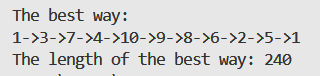
\includegraphics[]{комивояжер.png}
\centering
\caption{Результат работы программы}
\end{figure}
\chapter{Задача о назначениях}
Решить задачу о назначениях с помощью венгерского алгоритма.\\
Имеется n видов ресурсов, которые нужно распределить на n объектов, n = 10.\\
$c_{ij}$ - затраты, связанные с назначением i-го ресурса на j-й объект.\\
Каждый ресурс назначается ровно один раз и каждому объекту приписывается ровно один ресурс.\\
Требуется минимизировать стоимость назначений.

\begin{center}
    \begin{tabular}{|a | c | c | c | c | c | c | c | c | c | c|} 
         \hline
         \rowcolor{LightGray}
            & 1 & 2 & 3 & 4 & 5 & 6 & 7 & 8 & 9 & 10\\
         \hline
            1 & 1 & 3 & 6 & 4 & 7 & 1 & 8 & 2 & 8 & 3\\
         \hline
            2 & 1 & 6 & 4 & 9 & 8 & 3 & 5 & 7 & 1 & 2\\
         \hline
            3 & 8 & 1 & 5 & 9 & 3 & 6 & 4 & 7 & 7 & 9\\
         \hline
            4 & 3 & 6 & 1 & 9 & 2 & 4 & 5 & 8 & 3 & 5\\
        \hline
            5 & 2 & 7 & 9 & 4 & 1 & 2 & 8 & 9 & 5 & 2\\
         \hline
            6 & 7 & 1 & 8 & 6 & 3 & 2 & 4 & 7 & 9 & 5\\
         \hline
            7 & 6 & 8 & 5 & 9 & 2 & 4 & 7 & 1 & 2 & 3\\
         \hline
            8 & 2 & 4 & 7 & 5 & 9 & 1 & 4 & 8 & 7 & 3\\
        \hline
            9 & 7 & 1 & 6 & 9 & 3 & 2 & 5 & 3 & 4 & 2\\
         \hline
            10 & 6 & 4 & 7 & 5 & 9 & 4 & 5 & 8 & 1 & 3\\
        \hline
    \end{tabular}
\end{center}

\begin{center}
    {\bf
    Решение:}
\end{center}

\begin{center}
    \begin{tabular}{|a | c | c | c | c | c | c | c | c | c | c | g|} 
         \hline
         \rowcolor{LightGray}
            & 1 & 2 & 3 & 4 & 5 & 6 & 7 & 8 & 9 & 10 & min\\
         \hline
            1 & 1 & 3 & 6 & 4 & 7 & 1 & 8 & 2 & 8 & 3 & 1\\
         \hline
            2 & 1 & 6 & 4 & 9 & 8 & 3 & 5 & 7 & 1 & 2 & 1\\
         \hline
            3 & 8 & 1 & 5 & 9 & 3 & 6 & 4 & 7 & 7 & 9 & 1\\
         \hline
            4 & 3 & 6 & 1 & 9 & 2 & 4 & 5 & 8 & 3 & 5 & 1\\
        \hline
            5 & 2 & 7 & 9 & 4 & 1 & 2 & 8 & 9 & 5 & 2 & 1\\
         \hline
            6 & 7 & 1 & 8 & 6 & 3 & 2 & 4 & 7 & 9 & 5 & 1\\
         \hline
            7 & 6 & 8 & 5 & 9 & 2 & 4 & 7 & 1 & 2 & 3 & 1\\
         \hline
            8 & 2 & 4 & 7 & 5 & 9 & 1 & 4 & 8 & 7 & 3 & 1\\
        \hline
            9 & 7 & 1 & 6 & 9 & 3 & 2 & 5 & 3 & 4 & 2 & 1\\
         \hline
            10 & 6 & 4 & 7 & 5 & 9 & 4 & 5 & 8 & 1 & 3 & 1\\
        \hline
    \end{tabular}
\end{center}

\begin{center}
    \begin{tabular}{|a | c | c | c | c | c | c | c | c | c | c|} 
         \hline
         \rowcolor{LightGray}
            & 1 & 2 & 3 & 4 & 5 & 6 & 7 & 8 & 9 & 10\\
         \hline
            1 & 0 & 2 & 5 & 3 & 6 & 0 & 7 & 1 & 7 & 2\\
         \hline
            2 & 0 & 5 & 3 & 8 & 7 & 2 & 4 & 6 & 0 & 1\\
         \hline
            3 & 7 & 0 & 4 & 8 & 2 & 5 & 3 & 6 & 6 & 8\\
         \hline
            4 & 2 & 5 & 0 & 8 & 1 & 3 & 4 & 7 & 2 & 4\\
        \hline
            5 & 1 & 6 & 8 & 3 & 0 & 1 & 7 & 8 & 4 & 1\\
         \hline
            6 & 6 & 0 & 7 & 5 & 2 & 1 & 3 & 6 & 8 & 4\\
         \hline
            7 & 5 & 7 & 4 & 8 & 1 & 3 & 6 & 0 & 1 & 2\\
         \hline
            8 & 1 & 3 & 6 & 4 & 8 & 0 & 3 & 7 & 6 & 2\\
        \hline
            9 & 6 & 0 & 5 & 8 & 2 & 1 & 4 & 2 & 3 & 1\\
         \hline
            10 & 5 & 3 & 6 & 4 & 8 & 3 & 4 & 7 & 0 & 2\\
        \hline
        \rowcolor{LightBlue}
            min & 0 & 0 & 0 & 3 & 0 & 0 & 3 & 0 & 0 & 1\\
         \hline
    \end{tabular}
\end{center}

\begin{center}
    \begin{tabular}{|a | c | c | c | c | c | c | c | c | c | c|} 
         \hline
         \rowcolor{LightGray}
            & 1 & 2 & 3 & 4 & 5 & 6 & 7 & 8 & 9 & 10\\
         \hline
            1 & 0 & 2 & 5 & 0 & 6 & 0 & 4 & 1 & 7 & 1\\
         \hline
            2 & 0 & 5 & 3 & 5 & 7 & 2 & 1 & 6 & 0 & 0\\
         \hline
            3 & 7 & 0 & 4 & 5 & 2 & 5 & 0 & 6 & 6 & 7\\
         \hline
            4 & 2 & 5 & 0 & 5 & 1 & 3 & 1 & 7 & 2 & 3\\
        \hline
            5 & 1 & 6 & 8 & 0 & 0 & 1 & 4 & 8 & 4 & 0\\
         \hline
            6 & 6 & 0 & 7 & 2 & 2 & 1 & 0 & 6 & 8 & 3\\
         \hline
            7 & 5 & 7 & 4 & 5 & 1 & 3 & 3 & 0 & 1 & 1\\
         \hline
            8 & 1 & 3 & 6 & 1 & 8 & 0 & 0 & 7 & 6 & 1\\
        \hline
            9 & 6 & 0 & 5 & 5 & 2 & 1 & 1 & 2 & 3 & 0\\
         \hline
            10 & 5 & 3 & 6 & 1 & 8 & 3 & 1 & 7 & 0 & 1\\
        \hline
    \end{tabular}
\end{center}

\begin{center}
    \begin{tabular}{|a | c | c | c | c | c | c | c | c | c | c|} 
         \hline
         \rowcolor{LightGray}
            & 1 & 2 & 3 & 4 & 5 & 6 & 7 & 8 & 9 & 10\\
         \hline
            1 & 0 & 2 & 5 & \cellcolor{Beige}0 & 6 & 0 & 4 & 1 & 7 & 1\\
         \hline
            2 & \cellcolor{Beige}0 & 5 & 3 & 5 & 7 & 2 & 1 & 6 & 0 & 0\\
         \hline
            3 & 7 & \cellcolor{Beige}0 & 4 & 5 & 2 & 5 & 0 & 6 & 6 & 7\\
         \hline
            4 & 2 & 5 & \cellcolor{Beige}0 & 5 & 1 & 3 & 1 & 7 & 2 & 3\\
        \hline
            5 & 1 & 6 & 8 & 0 & \cellcolor{Beige}0 & 1 & 4 & 8 & 4 & 0\\
         \hline
            6 & 6 & 0 & 7 & 2 & 2 & 1 & \cellcolor{Beige}0 & 6 & 8 & 3\\
         \hline
            7 & 5 & 7 & 4 & 5 & 1 & 3 & 3 & \cellcolor{Beige}0 & 1 & 1\\
         \hline
            8 & 1 & 3 & 6 & 1 & 8 & \cellcolor{Beige}0 & 0 & 7 & 6 & 1\\
        \hline
            9 & 6 & 0 & 5 & 5 & 2 & 1 & 1 & 2 & 3 & \cellcolor{Beige}0\\
         \hline
            10 & 5 & 3 & 6 & 1 & 8 & 3 & 1 & 7 & \cellcolor{Beige}0 & 1\\
        \hline
    \end{tabular}
\end{center}

Назначение полное $\implies$ оптимальное.\\
Стоимость оптимального назначения:\\
\small{$(1 + 3) + (1 + 0) + (1 + 0) + (1 + 0) + (1 + 0) + (1 + 3) + (1 + 0) + (1 + 0) + (1 + 1) + (1 + 0) = 17$}\\

{\bfОтвет:} Стоимость оптимального назначения равна 17\\

{\bfКод программы на Python для решения задачи о назначениях}

\begin{lstlisting}
import numpy as np
from scipy.optimize import linear_sum_assignment

cost_matrix = np.array ([
    [1, 3, 6, 4, 7, 1, 8, 2, 8, 3],
    [1, 6, 4, 9, 8, 3, 5, 7, 1, 2],
    [8, 1, 5, 9, 3, 6, 4, 7, 7, 9],
    [3, 6, 1, 9, 2, 4, 5, 8, 3, 5],
    [2, 7, 9, 4, 1, 2, 8, 9, 5, 2],
    [7, 1, 8, 6, 3, 2, 4, 7, 9, 5],
    [6, 8, 5, 9, 2, 4, 7, 1, 2, 3],
    [2, 4, 7, 5, 9, 1, 4, 8, 7, 3],
    [7, 1, 6, 9, 3, 2, 5, 3, 4, 2],
    [6, 4, 7, 5, 9, 4, 5, 8, 1, 3]
])

row_ind, col_ind = linear_sum_assignment(cost_matrix)

optimal_cost = cost_matrix[row_ind, col_ind].sum()

print("Optimal cost: ", optimal_cost)
print("\nAssignments:")

for i in range(10):
    print('(', row_ind[i - 1] + 1, ';', col_ind[i - 1] + 1, ')')
\end{lstlisting}

\begin{figure}[ht]
\centering
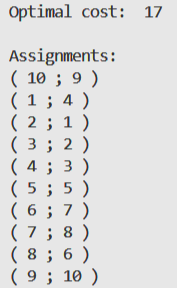
\includegraphics[]{венгерский метод.png}
\centering
\caption{Результат работы программы}
\end{figure}

\chapter{Задача о распределении ресурсов} 
Имеется однородный ресурс в количестве S = 6 единиц, который должен быть распределен между N = 6 предприятиями.\\
Использование i-м предприятием $x_{i}$ единиц ресурса дает доход, определяемый значением нелинейной функции $f_{i}(x_{i})$ (см. таблицу). Требуется найти распределение ресурсов между предприятиями, обеспечивающее максимальный доход.

\begin{center}
    \begin{tabular}{|a | c | c | c | c | c | c|} 
        \hline
             & \multicolumn{6}{c|}{предприятия}\\
         \hline
         \rowcolor{LightGray}
            & 1 & 2 & 3 & 4 & 5 & 6\\
        \hline
            0 & 0 & 0 & 0 & 0 & 0 & 0 \\
         \hline
            1 & 3 & 1 & 2 & 4 & 6 & 5 \\
         \hline
            2 & 4 & 5 & 8 & 1 & 4 & 4 \\
         \hline
            3 & 6 & 4 & 3 & 7 & 7 & 3 \\
         \hline
            4 & 2 & 7 & 1 & 2 & 3 & 2 \\
        \hline
            5 & 5 & 3 & 5 & 9 & 5 & 1 \\
         \hline
            6 & 6 & 1 & 7 & 4 & 2 & 4 \\
         \hline
    \end{tabular}
\end{center}

\begin{center}
    {\bf
    Решение:}
\end{center}

\begin{center}
    $F = \displaystyle \sum_{i=1}^{6} f_{i}(x_{i}) \rightarrow max$\\
    $\displaystyle \sum_{i=1}^{6} x_{i} = 6, x_{i} \ge 0, i = \overline{1, 6}$
\end{center}

\subsection*{1)} Оценим эффективность выделения ресурса на 1-е предприятие:\\
$\varphi_1(x) = \stackrel[0 \le x_1 \le x]{}{max}  \{f_1(x_1)\}$\\
$\varphi_1(0) = 0, x_1^0 = 0$\\
$\varphi_1(1) = max\{0; 3\} = 3, x_1^0 = 1$\\
$\varphi_1(2) = max\{0; 3; 4\} = 4, x_1^0 = 2$\\
$\varphi_1(3) = max\{0; 3; 4; 6\} = 6, x_1^0 = 3$\\
$\varphi_1(4) = max\{0; 3; 4; 6; 2\} = 6, x_1^0 = 3$\\
$\varphi_1(5) = max\{0; 3; 4; 6; 2; 5\} = 6, x_1^0 = 3$\\
$\varphi_1(6) = max\{0; 3; 4; 6; 2; 5; 6\} = 6, x_1^0 = 3$\\

\subsection*{2)} Оценим эффективность выделения ресурса на 1-е, 2-е предприятия:\\
$\varphi_2(x) = \stackrel[0 \le x_2 \le x]{}{max}  \{f_2(x_2) + \varphi_1(x - x_2)\}$\\

$\varphi_2(0) = 0, x_2^0 = 0$\\

$\varphi_2(1) = max \begin{Bmatrix}
    f_2(0) + \varphi_1(1 - 0) \\
    f_2(1) + \varphi_1(1 - 1) \\
\end{Bmatrix} = max \begin{Bmatrix}
    0 + 3 \\
    1 + 0 \\
\end{Bmatrix} = 3, x_2^0 = 0$\\

$\varphi_2(2) = max \begin{Bmatrix}
    f_2(0) + \varphi_1(2 - 0) \\
    f_2(1) + \varphi_1(2 - 1) \\
    f_2(2) + \varphi_1(2 - 2) \\
\end{Bmatrix} = max \begin{Bmatrix}
    0 + 4 \\
    1 + 3 \\
    5 + 0 \\
\end{Bmatrix} = 5, x_2^0 = 2$\\

$\varphi_2(3) = max \begin{Bmatrix}
    f_2(0) + \varphi_1(3 - 0) \\
    f_2(1) + \varphi_1(3 - 1) \\
    f_2(2) + \varphi_1(3 - 2) \\
    f_2(3) + \varphi_1(3 - 3) \\
\end{Bmatrix} = max \begin{Bmatrix}
    0 + 6 \\
    1 + 4 \\
    5 + 3 \\
    4 + 0 \\
\end{Bmatrix} = 8, x_2^0 = 2$\\

$\varphi_2(4) = max \begin{Bmatrix}
    f_2(0) + \varphi_1(4 - 0) \\
    f_2(1) + \varphi_1(4 - 1) \\
    f_2(2) + \varphi_1(4 - 2) \\
    f_2(3) + \varphi_1(4 - 3) \\
    f_2(4) + \varphi_1(4 - 4) \\
\end{Bmatrix} = max \begin{Bmatrix}
    0 + 6 \\
    1 + 6 \\
    5 + 4 \\
    4 + 3 \\
    7 + 0 \\
\end{Bmatrix} = 9, x_2^0 = 2$\\

$\varphi_2(5) = max \begin{Bmatrix}
    f_2(0) + \varphi_1(5 - 0) \\
    f_2(1) + \varphi_1(5 - 1) \\
    f_2(2) + \varphi_1(5 - 2) \\
    f_2(3) + \varphi_1(5 - 3) \\
    f_2(4) + \varphi_1(5 - 4) \\
    f_2(5) + \varphi_1(5 - 5) \\
\end{Bmatrix} = max \begin{Bmatrix}
    0 + 6 \\
    1 + 6 \\
    5 + 6 \\
    4 + 4 \\
    7 + 3 \\
    3 + 0 \\
\end{Bmatrix} = 11, x_2^0 = 2$\\

$\varphi_2(6) = max \begin{Bmatrix}
    f_2(0) + \varphi_1(6 - 0) \\
    f_2(1) + \varphi_1(6 - 1) \\
    f_2(2) + \varphi_1(6 - 2) \\
    f_2(3) + \varphi_1(6 - 3) \\
    f_2(4) + \varphi_1(6 - 4) \\
    f_2(5) + \varphi_1(6 - 5) \\
    f_2(6) + \varphi_1(6 - 6) \\
\end{Bmatrix} = max \begin{Bmatrix}
    0 + 6 \\
    1 + 6 \\
    5 + 6 \\
    4 + 6 \\
    7 + 4 \\
    3 + 3 \\
    1 + 0 \\
\end{Bmatrix} = 11, x_2^0 = 2$\\


\subsection*{3)} Оценим эффективность выделения ресурса на 1-е, 2-е, 3-е предприятия:\\
$\varphi_3(x) = \stackrel[0 \le x_3 \le x]{}{max}  \{f_3(x_3) + \varphi_2(x - x_3)\}$\\

$\varphi_3(0) = 0, x_3^0 = 0$\\

$\varphi_3(1) = max \begin{Bmatrix}
    f_3(0) + \varphi_2(1 - 0) \\
    f_3(1) + \varphi_2(1 - 1) \\
\end{Bmatrix} = max \begin{Bmatrix}
    0 + 3 \\
    2 + 0 \\
\end{Bmatrix} = 3, x_3^0 = 0$\\

$\varphi_3(2) = max \begin{Bmatrix}
    f_3(0) + \varphi_2(2 - 0) \\
    f_3(1) + \varphi_2(2 - 1) \\
    f_3(2) + \varphi_2(2 - 2) \\
\end{Bmatrix} = max \begin{Bmatrix}
    0 + 5 \\
    2 + 3 \\
    8 + 0 \\
\end{Bmatrix} = 5, x_3^0 = 0$\\

$\varphi_3(3) = max \begin{Bmatrix}
    f_3(0) + \varphi_2(3 - 0) \\
    f_3(1) + \varphi_2(3 - 1) \\
    f_3(2) + \varphi_2(3 - 2) \\
    f_3(3) + \varphi_2(3 - 3) \\
\end{Bmatrix} = max \begin{Bmatrix}
    0 + 8 \\
    2 + 5 \\
    8 + 3 \\
    3 + 0 \\
\end{Bmatrix} = 11, x_3^0 = 2$\\

$\varphi_3(4) = max \begin{Bmatrix}
    f_3(0) + \varphi_2(4 - 0) \\
    f_3(1) + \varphi_2(4 - 1) \\
    f_3(2) + \varphi_2(4 - 2) \\
    f_3(3) + \varphi_2(4 - 3) \\
    f_3(4) + \varphi_2(4 - 4) \\
\end{Bmatrix} = max \begin{Bmatrix}
    0 + 9 \\
    2 + 8 \\
    8 + 5 \\
    3 + 3 \\
    1 + 0 \\
\end{Bmatrix} = 13, x_3^0 = 2$\\

$\varphi_3(5) = max \begin{Bmatrix}
    f_3(0) + \varphi_2(5 - 0) \\
    f_3(1) + \varphi_2(5 - 1) \\
    f_3(2) + \varphi_2(5 - 2) \\
    f_3(3) + \varphi_2(5 - 3) \\
    f_3(4) + \varphi_2(5 - 4) \\
    f_3(5) + \varphi_2(5 - 5) \\
\end{Bmatrix} = max \begin{Bmatrix}
    0 + 11 \\
    2 + 9 \\
    8 + 8 \\
    3 + 5 \\
    1 + 3 \\
    5 + 0 \\
\end{Bmatrix} = 16, x_3^0 = 2$\\

$\varphi_3(6) = max \begin{Bmatrix}
    f_3(0) + \varphi_2(6 - 0) \\
    f_3(1) + \varphi_2(6 - 1) \\
    f_3(2) + \varphi_2(6 - 2) \\
    f_3(3) + \varphi_2(6 - 3) \\
    f_3(4) + \varphi_2(6 - 4) \\
    f_3(5) + \varphi_2(6 - 5) \\
    f_3(6) + \varphi_2(6 - 6) \\
\end{Bmatrix} = max \begin{Bmatrix}
    0 + 11 \\
    2 + 11 \\
    8 + 9 \\
    3 + 8 \\
    1 + 5 \\
    5 + 3 \\
    7 + 0 \\
\end{Bmatrix} = 17, x_3^0 = 2$\\


\subsection*{4)} Оценим эффективность выделения ресурса на 1-е, 2-е, 3-е, 4-е предприятия:\\
$\varphi_4(x) = \stackrel[0 \le x_4 \le x]{}{max}  \{f_4(x_4) + \varphi_3(x - x_4)\}$\\

$\varphi_4(0) = 0, x_4^0 = 0$\\

$\varphi_4(1) = max \begin{Bmatrix}
    f_4(0) + \varphi_3(1 - 0) \\
    f_4(1) + \varphi_3(1 - 1) \\
\end{Bmatrix} = max \begin{Bmatrix}
    0 + 3 \\
    4 + 0 \\
\end{Bmatrix} = 4, x_4^0 = 1$\\

$\varphi_4(2) = max \begin{Bmatrix}
    f_4(0) + \varphi_3(2 - 0) \\
    f_4(1) + \varphi_3(2 - 1) \\
    f_4(2) + \varphi_3(2 - 2) \\
\end{Bmatrix} = max \begin{Bmatrix}
    0 + 5 \\
    4 + 3 \\
    1 + 0 \\
\end{Bmatrix} = 7, x_4^0 = 1$\\

$\varphi_4(3) = max \begin{Bmatrix}
    f_4(0) + \varphi_3(3 - 0) \\
    f_4(1) + \varphi_3(3 - 1) \\
    f_4(2) + \varphi_3(3 - 2) \\
    f_4(3) + \varphi_3(3 - 3) \\
\end{Bmatrix} = max \begin{Bmatrix}
    0 + 11 \\
    4 + 5 \\
    1 + 3 \\
    7 + 0 \\
\end{Bmatrix} = 11, x_4^0 = 0$\\

$\varphi_4(4) = max \begin{Bmatrix}
    f_4(0) + \varphi_3(4 - 0) \\
    f_4(1) + \varphi_3(4 - 1) \\
    f_4(2) + \varphi_3(4 - 2) \\
    f_4(3) + \varphi_3(4 - 3) \\
    f_4(4) + \varphi_3(4 - 4) \\
\end{Bmatrix} = max \begin{Bmatrix}
    0 + 13 \\
    4 + 11 \\
    1 + 5 \\
    7 + 3 \\
    2 + 0 \\
\end{Bmatrix} = 15, x_4^0 = 1$\\

$\varphi_4(5) = max \begin{Bmatrix}
    f_4(0) + \varphi_3(5 - 0) \\
    f_4(1) + \varphi_3(5 - 1) \\
    f_4(2) + \varphi_3(5 - 2) \\
    f_4(3) + \varphi_3(5 - 3) \\
    f_4(4) + \varphi_3(5 - 4) \\
    f_4(5) + \varphi_3(5 - 5) \\
\end{Bmatrix} = max \begin{Bmatrix}
    0 + 16 \\
    4 + 13 \\
    1 + 11 \\
    7 + 5 \\
    2 + 3 \\
    9 + 0 \\
\end{Bmatrix} = 17, x_4^0 = 1$\\

$\varphi_4(6) = max \begin{Bmatrix}
    f_4(0) + \varphi_3(6 - 0) \\
    f_4(1) + \varphi_3(6 - 1) \\
    f_4(2) + \varphi_3(6 - 2) \\
    f_4(3) + \varphi_3(6 - 3) \\
    f_4(4) + \varphi_3(6 - 4) \\
    f_4(5) + \varphi_3(6 - 5) \\
    f_4(6) + \varphi_3(6 - 6) \\
\end{Bmatrix} = max \begin{Bmatrix}
    0 + 17 \\
    4 + 16 \\
    1 + 13 \\
    7 + 11 \\
    2 + 5 \\
    9 + 3 \\
    4 + 0 \\
\end{Bmatrix} = 20, x_4^0 = 1$\\


\subsection*{5)} Оценим эффективность выделения ресурса на 1-е, 2-е, 3-е, 4-е, 5-е предприятия:\\
$\varphi_5(x) = \stackrel[0 \le x_5 \le x]{}{max}  \{f_5(x_5) + \varphi_4(x - x_5)\}$\\

$\varphi_5(0) = 0, x_5^0 = 0$\\

$\varphi_5(1) = max \begin{Bmatrix}
    f_5(0) + \varphi_4(1 - 0) \\
    f_5(1) + \varphi_4(1 - 1) \\
\end{Bmatrix} = max \begin{Bmatrix}
    0 + 4 \\
    6 + 0 \\
\end{Bmatrix} = 6, x_5^0 = 1$\\

$\varphi_5(2) = max \begin{Bmatrix}
    f_5(0) + \varphi_4(2 - 0) \\
    f_5(1) + \varphi_4(2 - 1) \\
    f_5(2) + \varphi_4(2 - 2) \\
\end{Bmatrix} = max \begin{Bmatrix}
    0 + 7 \\
    6 + 4 \\
    4 + 0 \\
\end{Bmatrix} = 10, x_5^0 = 1$\\

$\varphi_5(3) = max \begin{Bmatrix}
    f_5(0) + \varphi_4(3 - 0) \\
    f_5(1) + \varphi_4(3 - 1) \\
    f_5(2) + \varphi_4(3 - 2) \\
    f_5(3) + \varphi_4(3 - 3) \\
\end{Bmatrix} = max \begin{Bmatrix}
    0 + 11 \\
    6 + 7 \\
    4 + 4 \\
    7 + 0 \\
\end{Bmatrix} = 13, x_5^0 = 1$\\

$\varphi_5(4) = max \begin{Bmatrix}
    f_5(0) + \varphi_4(4 - 0) \\
    f_5(1) + \varphi_4(4 - 1) \\
    f_5(2) + \varphi_4(4 - 2) \\
    f_5(3) + \varphi_4(4 - 3) \\
    f_5(4) + \varphi_4(4 - 4) \\
\end{Bmatrix} = max \begin{Bmatrix}
    0 + 15 \\
    6 + 11 \\
    4 + 7 \\
    7 + 4 \\
    3 + 0 \\
\end{Bmatrix} = 17, x_5^0 = 1$\\

$\varphi_5(5) = max \begin{Bmatrix}
    f_5(0) + \varphi_4(5 - 0) \\
    f_5(1) + \varphi_4(5 - 1) \\
    f_5(2) + \varphi_4(5 - 2) \\
    f_5(3) + \varphi_4(5 - 3) \\
    f_5(4) + \varphi_4(5 - 4) \\
    f_5(5) + \varphi_4(5 - 5) \\
\end{Bmatrix} = max \begin{Bmatrix}
    0 + 17 \\
    6 + 15 \\
    4 + 11 \\
    7 + 7 \\
    3 + 4 \\
    5 + 0 \\
\end{Bmatrix} = 21, x_5^0 = 1$\\

$\varphi_5(6) = max \begin{Bmatrix}
    f_5(0) + \varphi_4(6 - 0) \\
    f_5(1) + \varphi_4(6 - 1) \\
    f_5(2) + \varphi_4(6 - 2) \\
    f_5(3) + \varphi_4(6 - 3) \\
    f_5(4) + \varphi_4(6 - 4) \\
    f_5(5) + \varphi_4(6 - 5) \\
    f_5(6) + \varphi_4(6 - 6) \\
\end{Bmatrix} = max \begin{Bmatrix}
    0 + 20 \\
    6 + 17 \\
    4 + 15 \\
    7 + 11 \\
    3 + 7 \\
    5 + 4 \\
    2 + 0 \\
\end{Bmatrix} = 23, x_5^0 = 1$\\


\subsection*{6)} Оценим эффективность выделения ресурса на 1-е, 2-е, 3-е, 4-е, 5-е, 6-е предприятия:\\
$\varphi_6(x) = \stackrel[0 \le x_6 \le x]{}{max}  \{f_6(x_6) + \varphi_5(x - x_6)\}$\\

$\varphi_6(0) = 0, x_6^0 = 0$\\

$\varphi_6(1) = max \begin{Bmatrix}
    f_6(0) + \varphi_5(1 - 0) \\
    f_6(1) + \varphi_5(1 - 1) \\
\end{Bmatrix} = max \begin{Bmatrix}
    0 + 6 \\
    5 + 0 \\
\end{Bmatrix} = 6, x_6^0 = 0$\\

$\varphi_6(2) = max \begin{Bmatrix}
    f_6(0) + \varphi_5(2 - 0) \\
    f_6(1) + \varphi_5(2 - 1) \\
    f_6(2) + \varphi_5(2 - 2) \\
\end{Bmatrix} = max \begin{Bmatrix}
    0 + 10 \\
    5 + 6 \\
    4 + 0 \\
\end{Bmatrix} = 11, x_6^0 = 1$\\

$\varphi_6(3) = max \begin{Bmatrix}
    f_6(0) + \varphi_5(3 - 0) \\
    f_6(1) + \varphi_5(3 - 1) \\
    f_6(2) + \varphi_5(3 - 2) \\
    f_6(3) + \varphi_5(3 - 3) \\
\end{Bmatrix} = max \begin{Bmatrix}
    0 + 13 \\
    5 + 10 \\
    4 + 6 \\
    3 + 0 \\
\end{Bmatrix} = 15, x_6^0 = 1$\\

$\varphi_6(4) = max \begin{Bmatrix}
    f_6(0) + \varphi_5(4 - 0) \\
    f_6(1) + \varphi_5(4 - 1) \\
    f_6(2) + \varphi_5(4 - 2) \\
    f_6(3) + \varphi_5(4 - 3) \\
    f_6(4) + \varphi_5(4 - 4) \\
\end{Bmatrix} = max \begin{Bmatrix}
    0 + 17 \\
    5 + 13 \\
    4 + 10 \\
    3 + 6 \\
    2 + 0 \\
\end{Bmatrix} = 18, x_6^0 = 1$\\

$\varphi_6(5) = max \begin{Bmatrix}
    f_6(0) + \varphi_5(5 - 0) \\
    f_6(1) + \varphi_5(5 - 1) \\
    f_6(2) + \varphi_5(5 - 2) \\
    f_6(3) + \varphi_5(5 - 3) \\
    f_6(4) + \varphi_5(5 - 4) \\
    f_6(5) + \varphi_5(5 - 5) \\
\end{Bmatrix} = max \begin{Bmatrix}
    0 + 21 \\
    5 + 17 \\
    4 + 13 \\
    3 + 10 \\
    2 + 6 \\
    1 + 0 \\
\end{Bmatrix} = 22, x_6^0 = 1$\\

$\varphi_6(6) = max \begin{Bmatrix}
    f_6(0) + \varphi_5(6 - 0) \\
    f_6(1) + \varphi_5(6 - 1) \\
    f_6(2) + \varphi_5(6 - 2) \\
    f_6(3) + \varphi_5(6 - 3) \\
    f_6(4) + \varphi_5(6 - 4) \\
    f_6(5) + \varphi_5(6 - 5) \\
    f_6(6) + \varphi_5(6 - 6) \\
\end{Bmatrix} = max \begin{Bmatrix}
    0 + 23 \\
    5 + 21 \\
    4 + 17 \\
    3 + 13 \\
    2 + 10 \\
    1 + 6 \\
    4 + 0 \\
\end{Bmatrix} = 26, x_6^0 = 1$\\

6-му предприятию: $x_6^0 = 1 \implies S = S - 1 = 6 - 1 = 5$\\
$\varphi_5(5)$ при $x_5^0 = 1 \implies$ 5-му предприятию: 1 $\implies S = S - 1 = 5 - 1 = 4$\\
$\varphi_4(4)$ при $x_4^0 = 1 \implies$ 4-му предприятию: 1 $\implies S = S - 1 = 4 - 1 = 3$\\
$\varphi_3(3)$ при $x_3^0 = 2 \implies$ 3-му предприятию: 2 $\implies S = S - 2 = 3 - 2 = 1$\\
$\varphi_2(1)$ при $x_2^0 = 0 \implies$ 2-му предприятию: 0 $\implies S = 1$\\
$\varphi_1(1)$ при $x_1^0 = 1 \implies$ 1-му предприятию: 1 $\implies S = 0$\\

$X^0 = (1, 0, 2, 1, 1, 1)$. Прибыль: 3 + 0 + 8 + 4 + 6 + 5 = 26\\

{\bfОтвет: }\\ Распределение ресурсов между предприятиями: $X^0 = (1, 0, 2, 1, 1, 1)$. Прибыль: 26\\
\newpage

{\bfКод программы на Python для решения задачи о распределении ресурсов}

\begin{lstlisting}
    resourse = [[0, 0, 0, 0, 0, 0],
    [3, 1, 2, 4, 6, 5],
    [4, 5, 8, 1, 4, 4],
    [6, 4, 3, 7, 7, 3],
    [2, 7, 1, 2, 3, 2],
    [5, 3, 5, 9, 5, 1],
    [6, 1, 7, 4, 2, 4]]

max_profit = 0
optimal = ""

for a_1 in range(7):
for a_2 in range(7-a_1):
for a_3 in range(7-a_1-a_2):
    for a_4 in range(7-a_1-a_2-a_3):
        for a_5 in range(7-a_1-a_2-a_3-a_4):
            for a_6 in range(7-a_1-a_2-a_3-a_4-a_5):
                profit = resourse[a_1][0] + resourse[a_2][1]
                profit += resourse[a_3][2] + resourse[a_4][3]
                profit += resourse[a_5][4] + resourse[a_6][5]
                if profit > max_profit:
                    max_profit = profit
                    optimal = str(a_1) + ", " + str(a_2) + ", "
                    optimal += str(a_3) + ", " + str(a_4) + ", "
                    optimal += str(a_5) + ", " + str(a_6)

\end{lstlisting}

\begin{figure}[h]
    \centering
    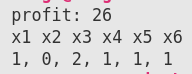
\includegraphics[]{9.png}
    \centering
    \caption{Результат работы программы}
\end{figure}
\chapter{Задача о рюкзаке}

Имеется рюкзак грузоподъемностью S = 20. Требуется заполнить его грузом, состоящим из предметов N = 6 различных типов таким образом, чтобы стоимость (ценность) всего груза была максимальной.

\begin{center}
    \begin{tabular}{|a | c | c | c | c | c | c|} 
         \hline
         \rowcolor{LightGray}
            С (предметы) & 1 & 2 & 3 & 4 & 5 & 6\\
        \hline
            Р (вес) & 9 & 5 & 8 & 7 & 4 & 6 \\
         \hline
            V (цена) & 12 & 9 & 14 & 10 & 16 & 8 \\
         \hline
    \end{tabular}
\end{center}

\begin{center}
    {\bf
    Решение:}
\end{center}

\begin{center}
    $W(x) = \displaystyle \sum_{i=1}^{6} x_{i}V_{i} \rightarrow max$\\
    $\displaystyle \sum_{i=1}^{6} x_{i}P_{i} \le 20, x_{i} = 0, 1,...$ - целочисленное\\
\end{center}

\subsection*{1)}
$W_1 (C)=\underset{0\le x_1 \le [\frac{25}{9}]}{max}\{x_1\cdot 12\}, x_1=0,1,2$

\begin{center}
    \begin{tabular}{|a|c|c|c|}
    \hline 
    C & 0-8 & 9-17 & 18-20\\ \hline
    $W_1 (C)$ & 0 & 12 & 24\\ \hline
    $x_1$ & 0 & 1 & 2\\ \hline
    \end{tabular}
\end{center}


\subsection*{2)}
$W_2 (S)=\underset{0\le x_2 \le [\frac{C}{5}]}{max}\{x_2\cdot 9 + W_1(C-x_2\cdot 5)\}, x_2=0,1,2,3,4$

\begin{center}
    \small
    \begin{tabular}{|a|c|c|c|c|c|c|c|c|}
    \hline 
    C & 0-4 & 5-8 & 9 & 10-13 & 14 & 15-18 & 19 & 20\\ \hline
    $W_2 (C)$ & 0 & 9 & 12 & 18 & 21 & 27 & 30 & 36 \\ \hline
    $x_2$ & 0 & 1 & 0 & 2 & 1 & 3 & 2 & 4 \\ \hline
    \end{tabular}
\end{center}



\subsection*{3)}
$W_3 (S)=\underset{0\le x_3 \le [\frac{C}{8}]}{max}\{x_3\cdot 14+W_2(C-x_3\cdot 8)\}, x_3=0,1,2$


\begin{flushleft}
    \small
    \begin{tabular}{|a|c|c|c|c|c|c|c|c|c|}
    \hline 
    C & 0-4 & 5-7 & 8-9 & 10-12 & 13-14 & 15 & 16-17 & 18-19 & 20\\ \hline
    $W_3 (C)$ & 0 & 9 & 14 & 18 & 23 & 27 & 28 & 32 & 36 \\ \hline
    $x_3$ & 0 & 0 & 1 & 0 & 1 & 0 & 2 & 1 & 0\\ \hline
    \end{tabular}
\end{flushleft}


\subsection*{4)}
$W_4 (S)=\underset{0\le x_4 \le [\frac{C}{7}]}{max}\{x_4\cdot 10+W_3(C-x_4\cdot 7)\}, x_4=0,1,2$

\begin{flushleft}
    \small
    \begin{tabular}{|a|c|c|c|c|c|c|c|c|c|c|c|}
    \hline 
    C & 0-4 & 5-6 & 7 & 8-9 & 10-11 & 12 & 13-14 & 15 & 16-17 & 18-19 & 20\\ \hline
    $W_3 (C)$ & 0 & 9 &  10& 14 & 18 & 19 & 23 & 27 & 28 & 32 & 36 \\ \hline
    $x_3$ & 0 & 0 & 1 & 0 & 0 & 1 & 0 & 0 & 0 & 0 & 0\\ \hline
    \end{tabular}
\end{flushleft}


\subsection*{5)}
$W_5 (S)=\underset{0\le x_5 \le [\frac{C}{4}]}{max}\{x_5\cdot 16+W_4(C-x_5\cdot 4)\}, x_5=\overline{0,5}$

\begin{flushleft}
    \small
    \begin{tabular}{|a|c|c|c|c|c|c|}
    \hline 
    C & 0-3 & 4-7 & 8-11 & 12-15 & 16-19 & 20 \\ \hline
    $W_3 (C)$ & 0 & 16 & 32 & 48 & 64 & 80 \\ \hline
    $x_3$ & 0 & 1 & 2 & 3 & 4 & 5 \\ \hline
    \end{tabular}
\end{flushleft}



\subsection*{6)}
$W_6 (S)=\underset{0\le x_6 \le [\frac{C}{6}]}{max}\{x_6\cdot 8+W_5(C-x_6\cdot 6)\}, x_5=\overline{0,3}$

\begin{flushleft}
    \small
    \begin{tabular}{|a|c|c|c|c|c|c|}
    \hline 
    C & 0-3 & 4-7 & 8-11 & 12-15 & 16-19 & 20 \\ \hline
    $W_3 (C)$ & 0 & 16 & 32 & 48 & 64 & 80 \\ \hline
    $x_3$ & 0 & 0 & 0 & 0 & 0 & 0 \\ \hline
    \end{tabular}
\end{flushleft}

Максимальная стоимость груза равна:$W_6(20)=80$\\
$
W_6(20)=80 \text{ при } x_6=0 \implies x_6^o=0\implies\\
W_6(20)=0\cdot 8 + W_5(20-0\cdot 6)=80\implies W_5(20)=80\implies\\
W_5(20)=80 \text{ при } x_5=5 \implies x_5^o=5\implies\\
W_5(20)=5\cdot 16 + W_4(20-5\cdot 4)=80\implies W_4(0)=0\implies\\
W_4(0)=0 \text{ при } x_4=0 \implies x_4^o=0\implies\\
W_3(0)=W_2(0)=W_1(0)=0 \text{ при } x_3= x_2 = x_1=0 \implies \\
x_3^o=x_2^o=x_1^o=0
$

{\bfОтвет:} максимальная стоимость груза равна 80, \\
опорный план: $x^0 = (0, 0, 0, 0, 5, 0)$

{\bfКод программы на Python для решения задачи о рюкзаке}

\begin{lstlisting}
    weights = [9, 5, 8, 7, 4, 6]
    values = [12, 9, 14, 10, 16, 8]
    capacity = 20
    
    max_profit = 0
    A = [0] * 6
    optimal = " "
    
    while A [0] * weights [0] <= capacity :
        A [1] = 0
        profit = A [0] * values [0]
        while A [1] * weights [1] <= capacity - A [0] * weights [0]:
            A [2] = 0
            while ( A [2] * weights [2] <= capacity - A [0] * weights [0] - A [1] * weights [1]) :
                A [3] = 0
                while ( A [3] * weights [3] <= capacity - A [0] * weights [0] - A [1] * weights [1] - A [2] * weights [2]) :
                    A [4] = 0
                    while ( A [4] * weights [4] <= capacity - A [0] * weights [0] - A [1] * weights [1] - A [2] * weights [2] - A [3] * weights [3]) :
                        A [5] = 0
                        while ( A [5] * weights [5] <= capacity - A [0] * weights [0] - A [1] * weights [1] - A [2] * weights [2] - A [3] * weights [3] - A [4] * weights [4]) :
                            profit = A [0] * values [0]
                            profit += A [1] * values [1]
                            profit += A [2] * values [2]
                            profit += A [3] * values [3]
                            profit += A [4] * values [4]
                            profit += A [5] * values [5]
                            if profit > max_profit :
                                max_profit = profit
                                optimal = str ( A [0]) + " , "
                                optimal += str ( A [1]) + " , "
                                optimal += str ( A [2]) + " , "
                                optimal += str ( A [3]) + " , "
                                optimal += str ( A [4]) + " , "
                                optimal += str ( A [5])
                            A [5] += 1
                        A [4] += 1
                    A [3] += 1
                A [2] += 1
            A [1] += 1
        A [0] += 1
    
    
    print ( " Max cost : " + str ( max_profit ) )
    print ( " x1 x2 x3 x4 x5 x6 " )
    print ( optimal )

\end{lstlisting}

\begin{figure}[h]
    \centering
    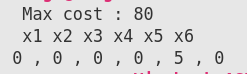
\includegraphics[]{10.png}
    \centering
    \caption{Результат работы программы}
\end{figure}


\end{document}